\chapter{Evaluación de la herramienta}
\label{cap:evaluacion}

En este capítulo se describirá la evaluación de la herramienta separando en una evaluación para el módulo de OCR, otra para el módulo de tests y una evaluación de la herramienta de forma conjunta(end to end testing).
En la parte de OCR se evaluará la librería utilizada, la mejora que proporciona la parte de preprocesamiento y la limpieza de caractéres basura utilizando distancia Levenshtein.
En la parte de tests se evaluará la precisión de los tests asegurándonos de que no exista casos que de un falso error en el test. 
De forma genérica se evaluará la herramienta con los resultados obtenidos ejecutando la herramienta midiendo la precisión.

\section{Pruebas y resultados de los OCR}
\label{sec:Evaluación_OCR}
En esta sección se hará una evaluación de los distintos OCRs para elegir la más conveniente para nuestra herramienta.
La evaluación se hará sobre las librerías de Tesseract, EasyOCR y OCRopus, son estas elegidas por su disponibilidad gratuita.

El objetivo de la evaluación es elegir el OCR que mejor se adapte a nuestras necesidades, lo que resalta la importancia de la precisión del OCR.
Para poder medir esa precisión, tendremos en cuenta el CER(\textit{Character Error Rate}). Además el tiempo también es un factor importante que tendremos en cuenta.

El CER(\textit{Character Error Rate}) es una métrica usada comúnmente para evaluar la precisión de un sistema de reconocimiento de caracteres u otros sistemas que transcriba texto. El valor se obtiene calculando el número de errores a nivel de carácter dividido por el número total de caracteres en el texto de referencia.
Los errores pueden ser debidos a:
\begin{enumerate}
	\item Sustituciones: Un carácter incorrecto reemplaza a uno correcto.
	\item Inserciones: Aparece un carácter extra que no debería estar.
	\item Eliminaciones: Falta un carácter que debería estar presente.
\end{enumerate}
La fórmula general para calcular el CER es:

$CER = \frac{S+D+I}{N} $ 

Donde:

S es el número de sustituciones.

D es el número de eliminaciones.

I es el número de inserciones.

N es el número total de caracteres en el texto de referencia.

El CER se expresa como un valor entre 0 y 1 (o como porcentaje), donde 0 significa que no hubo errores (transcripción perfecta) y 1 (o 100) indica que todos los caracteres son incorrectos.

La metodología seguida para la evaluación es la siguiente:

\begin{enumerate}
	\item Se hará la evaluación de forma independiente con las 3 librerías de OCR. Tesseract, EasyOCR y OCRopus.
	\item Se ha elegido 13 imágenes nombrados del 1 al 13 siendo la imagen 1(figura \ref{fig:imagen1}) el más simple y el 13(figura \ref{fig:imagen13}) el más complejo. Para la clasificación de simplificad de las imágenes se ha tenido en cuenta el número de caracteres a reconocer y la complejidad del fondo, entre ellas, el contraste y el número de geometrías.
	Las imágenes se pueden encontrar en el repositorio del trabajo\footnote{Repositorio github con las imágenes de evaluación: \url{https://github.com/Dewo2000/TFG-2024-2025/tree/main/OCRTests/images}}.
\begin{figure}[h]
	\centering
	\begin{minipage}{0.45\textwidth}
		\centering
		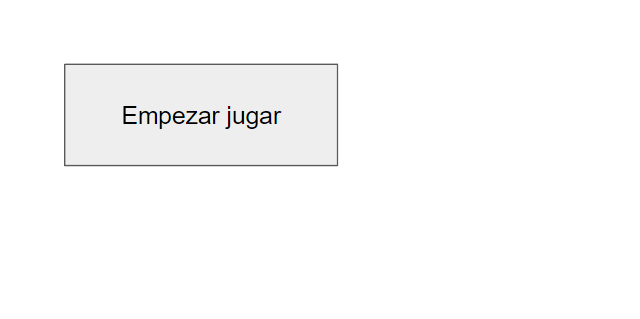
\includegraphics[width=\linewidth]{Imagenes/Evaluacion_OCR/1.png}
		\caption{Ejemplo de imagen simple.}
		\label{fig:imagen1}
	\end{minipage}
	\hfill
	\begin{minipage}{0.45\textwidth}
		\centering
		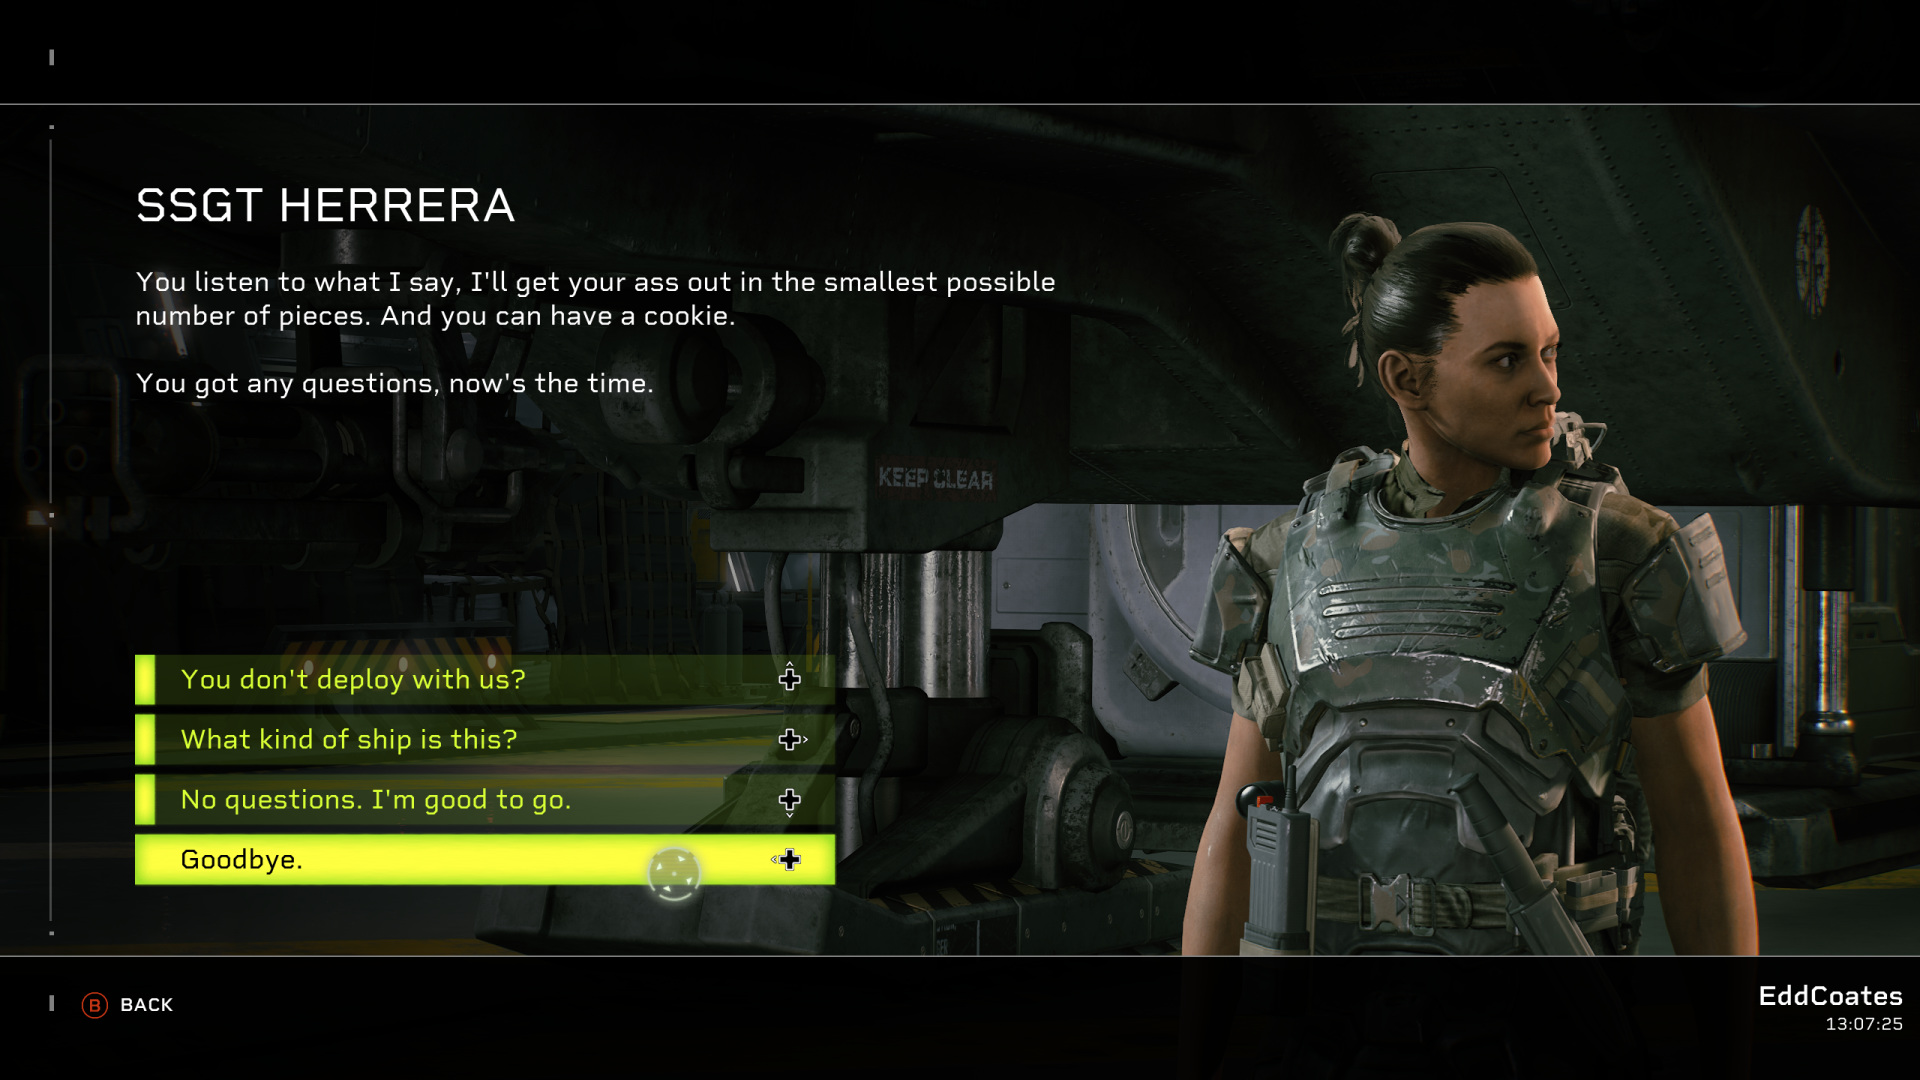
\includegraphics[width=\linewidth]{Imagenes/Evaluacion_OCR/13.png}
		\caption{Ejemplo de imagen complejo.}
		\label{fig:imagen13}
	\end{minipage}
\end{figure}
	\item Cada imagen será procesadas por el OCR utilizando el modelo por defecto de cada una de ellas.  
	\item Se utiliza la libreria Jiwer\footnote{(Jiwer Usage)\url {https://jitsi.github.io/jiwer/usage/}} en python para los cálculos de CER.
	\item Se ejecutará 6 veces el proceso de reconocimiento de cada OCR para sacar el tiempo medio de cada una.
\end{enumerate}


En los resultados de los OCR se encontrará un valor llamado CER medio, este valor se obtiene calculando el número total de errores a nivel de carácter encontrado en toda la batería de prueba divido entre el número total de caracteres de toda la batería de prueba.

Los resultados de los OCRs son las siguientes:
\begin{table}[H]
	\centering
	\caption{Resultado de CER de los OCR (Redondeado a 3 decimales)}
	\begin{tabular}{llll}
		\textbf{Imagen} & \textbf{Tesseract} & \textbf{EasyOCR} &\textbf{OCRopus} \\
		1  & 0.000 & 0.000 & 0.000 \\
		2  & 0.063 & 0.281 & 0.406 \\
		3  & 0.538 & 0.212 & 0.538 \\
		4  & 0.043 & 0.109 & 0.978 \\
		5  & 0.289 & 0.086 & 0.719 \\
		6  & 0.025 & 0.025 & 0.700 \\
		7  & 0.750 & 0.000 & 1.417 \\
		8  & 0.935 & 0.652 & 0.870 \\
		9  & 0.721 & 0.256 & 0.744 \\
		10 & 1.000 & 0.857 & 8.286 \\
		11 & 0.050 & 0.150 & 2.550 \\
		12 & 0.352 & 0.055 & 0.834 \\
		13 & 0.230 & 0.337 & 0.881 \\
		\textbf{CER medio} & \textbf{0.384}& \textbf{0.232} & \textbf{1.456}\\
	\end{tabular}
	\label{table:OCRResult}
\end{table}
\begin{table}[H]
	\centering
	\caption{Resultado de OCR en tiempo(ms)}
	\begin{tabular}{llll}
		\textbf{Iteración} & \textbf{Tesseract}& \textbf{EasyOCR}& \textbf{OCRopus} \\
		1  & 5539   & 204625 & 86213  \\
		2  & 5580   & 223809 & 90172  \\
		3  & 5539   & 216701 & 88290  \\
		4  & 5720   & 238900 & 83278  \\
		5  & 5602   & 216791 & 87810  \\
		6  & 5571   & 204502 & 88789  \\
		\textbf{Tiempo medio} & \textbf{5591}&\textbf{217554}&\textbf{87425} \\
	\end{tabular}
	\label{table:OCRResultTime}
\end{table}


Como podemos ver en la tabla \ref{table:OCRResult}, todos los OCRs han podido reconocer de forma exacta la imagen más simple y que todos han caido en la imagén 10. En cuanto las otras imágenes podemos observar que unas lo reconoce mejor Tesseract y otras EasyOCR por lo que ambos producen buenos resultados, en cuanto OCRopus, sus resultados ya no son tan buenos en comparación con las otras dos por lo que queda descartado. El OCR puede reconocer más caracteres del texto esperado por lo que el CER supera a 1 en algunos casos, lo llamamos caracteres basura que se explicará con más detalle en la sección \ref{subsec:Eliminación de caracter basura}. Aunque EasyOCR obtiene un mejor CER medio en los resultados (0.23) que Tesseract (0.38), Tesseract es muchísimo más rápido que EasyOCR teniendo un 211936 milisegundo de adelanto que equivale a 3 minutos y 50 segundos aproximadamente como podemos observar en la tabla \ref{table:OCRResultTime}. Por tanto decidimos seguir en adelante con Tesseract.



\section{Mejoras en el reconocimiento de texto en imágenes}
\label{sec:Mejoras en el reconocimiento}
Como podemos notar en los resultados del apartado anterior, la imagen 10 ha sido un reto para el CER de los OCRs, esto es debido a que el OCR reconoce como carácter geometrías del fondo y produce basura.Para solucionar esto, se plantea aplicar preprocesamiento a las imágenes y la limpieza del resultado usando distancia Levenshtein para mejorar la precisión del texto obtenido por el OCR disminuyendo el CER.

Para obtener más información sobre aquellos factores o características de las imágenes que puedan afectar al rendimiento y efectividad de la herramienta de OCR, se ha clasificado las imágenes en 5 categorías diferentes. La clasificación se ha hecho de forma subjetiva, de acuerdo a ciertas características de imágenes.
\begin{enumerate}
	\item Fondos simples(F.Simple)(Figura \ref{fig:Fsimple}). Imágenes donde la cantidad de geometrías del fondo son pocas o fáciles de reconocer(no se confunde con los caractéres).
	\begin{figure}[H]
		\centering
		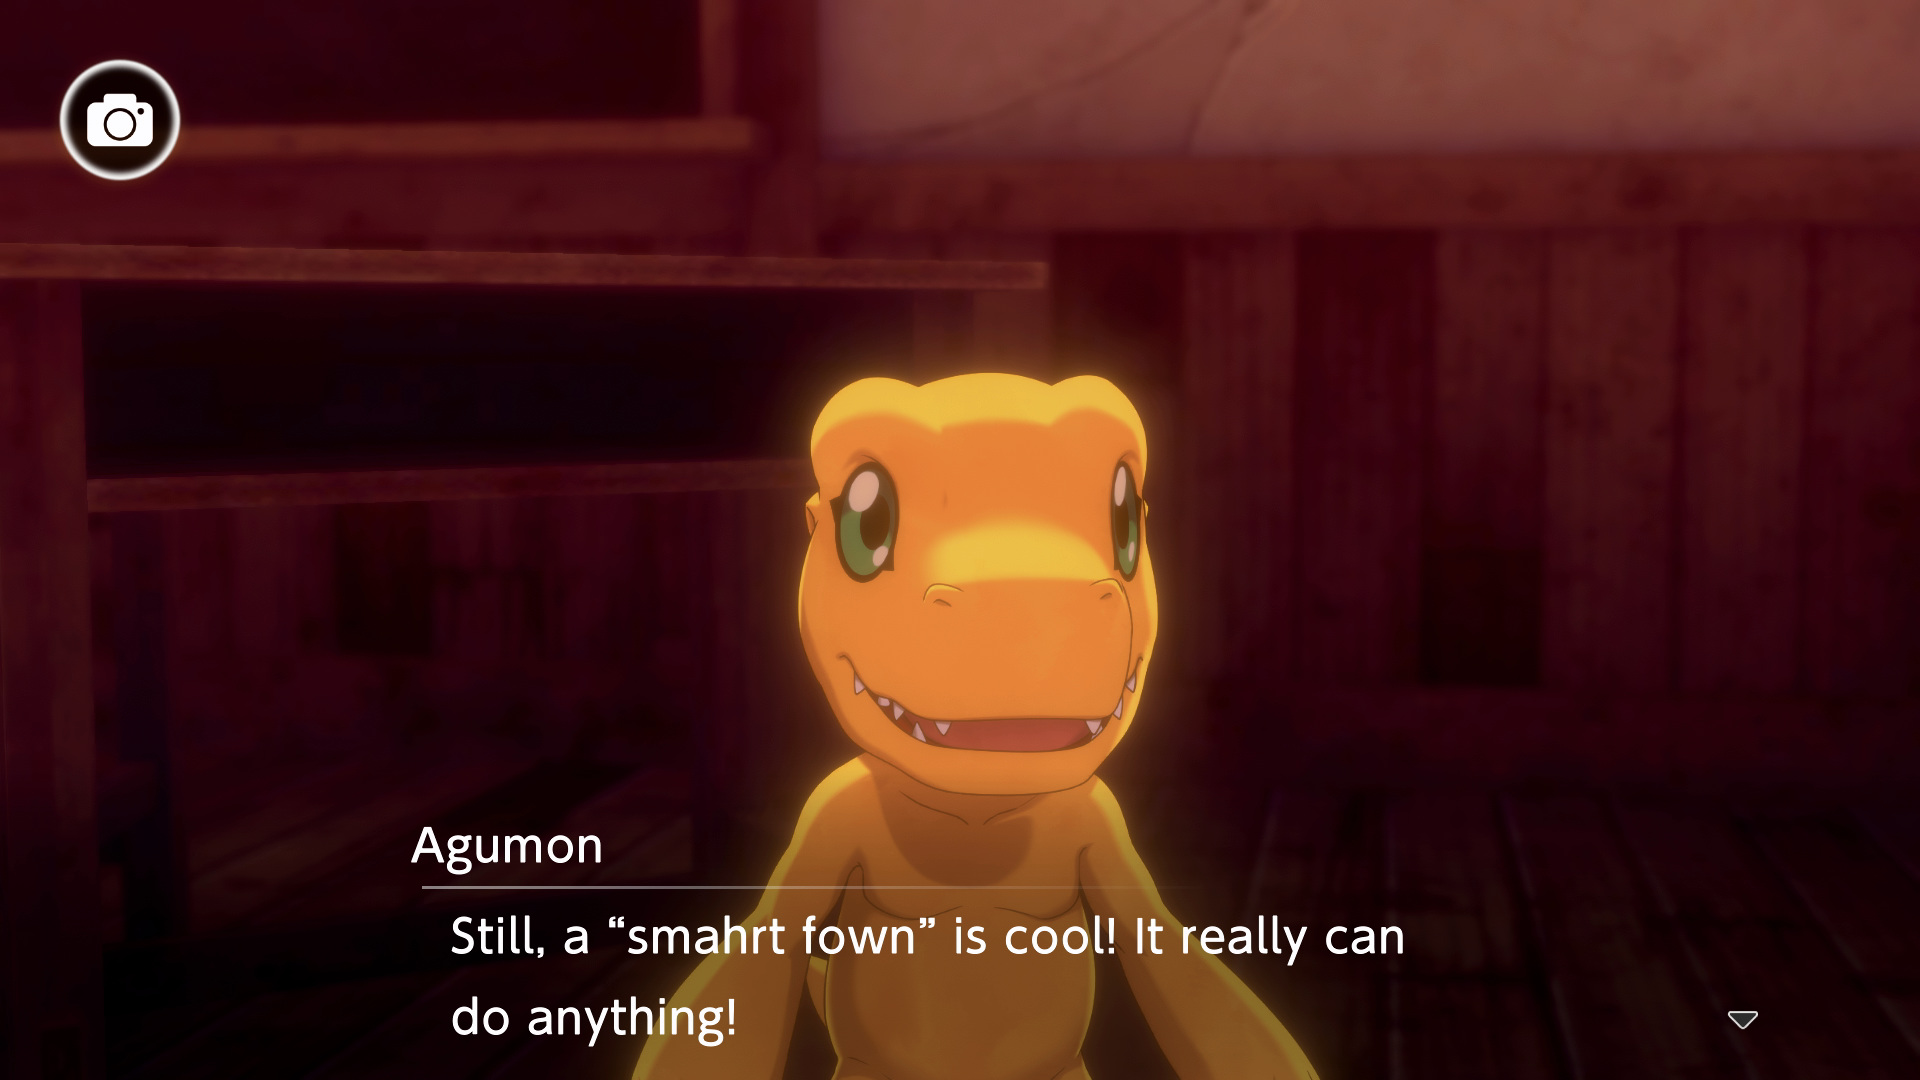
\includegraphics[width = 0.5\textwidth]{Imagenes/OCR/Simple.png}
		\caption{Ejemplo imagen fondos simples }
		\label{fig:Fsimple}
	\end{figure}
	
	\item Fondos complejos(F.Complejo)(Figura \ref{fig:Fcomplejo}). Imágenes donde la cantidad de geometrías del fondo son muchas o difíciles de reconocer(fácil de confundirse con los caractéres).
	\begin{figure}[H]
		\centering
		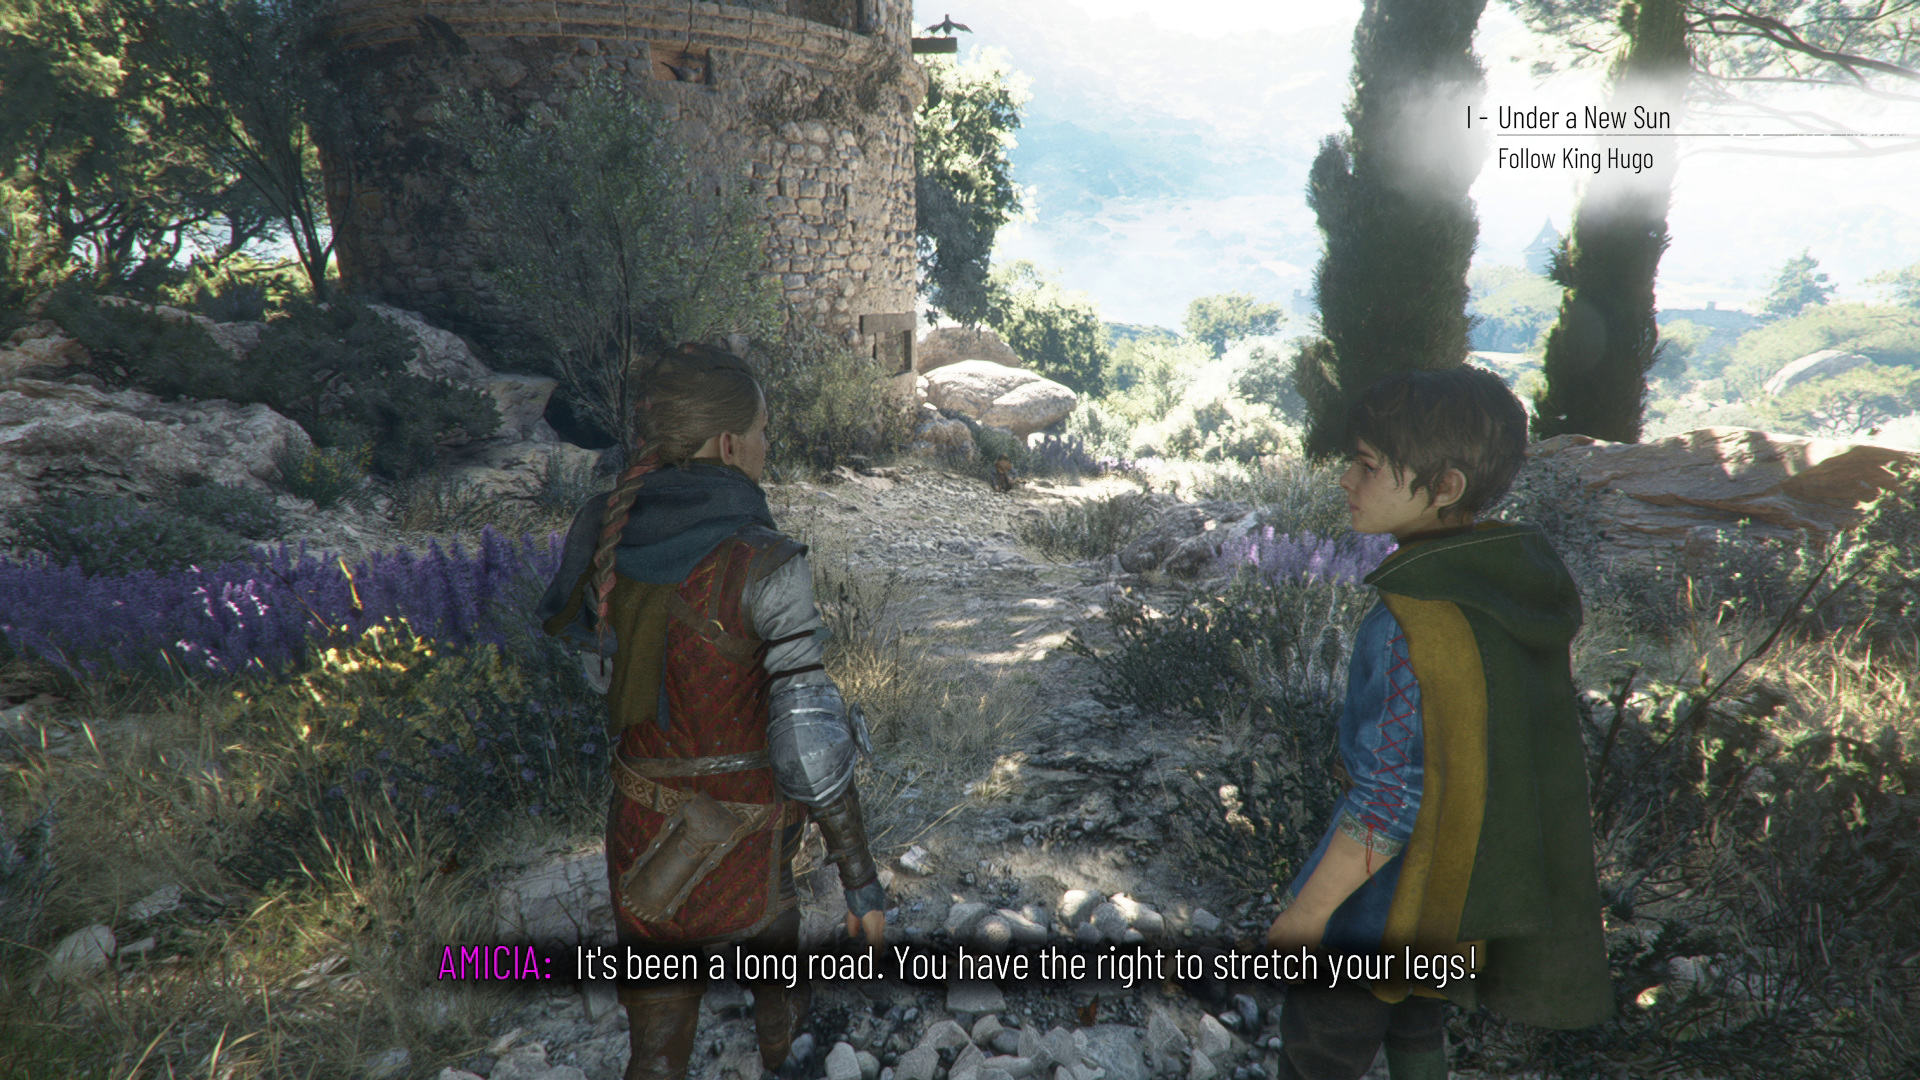
\includegraphics[width = 0.5\textwidth]{Imagenes/OCR/Complejo.png}
		\caption{Ejemplo imagen fondos complejos }
		\label{fig:Fcomplejo}
	\end{figure}
	\item PixelArt(PixelArt)(Figura \ref{fig:Pixelart}). Imágenes donde el fondo y las letras tiene un estilo pixelart. Como las imágenes son píxeladas(cuadrado de color que forman formas y texto), supone un reto para el OCR.
	\begin{figure}[H]
		\centering
		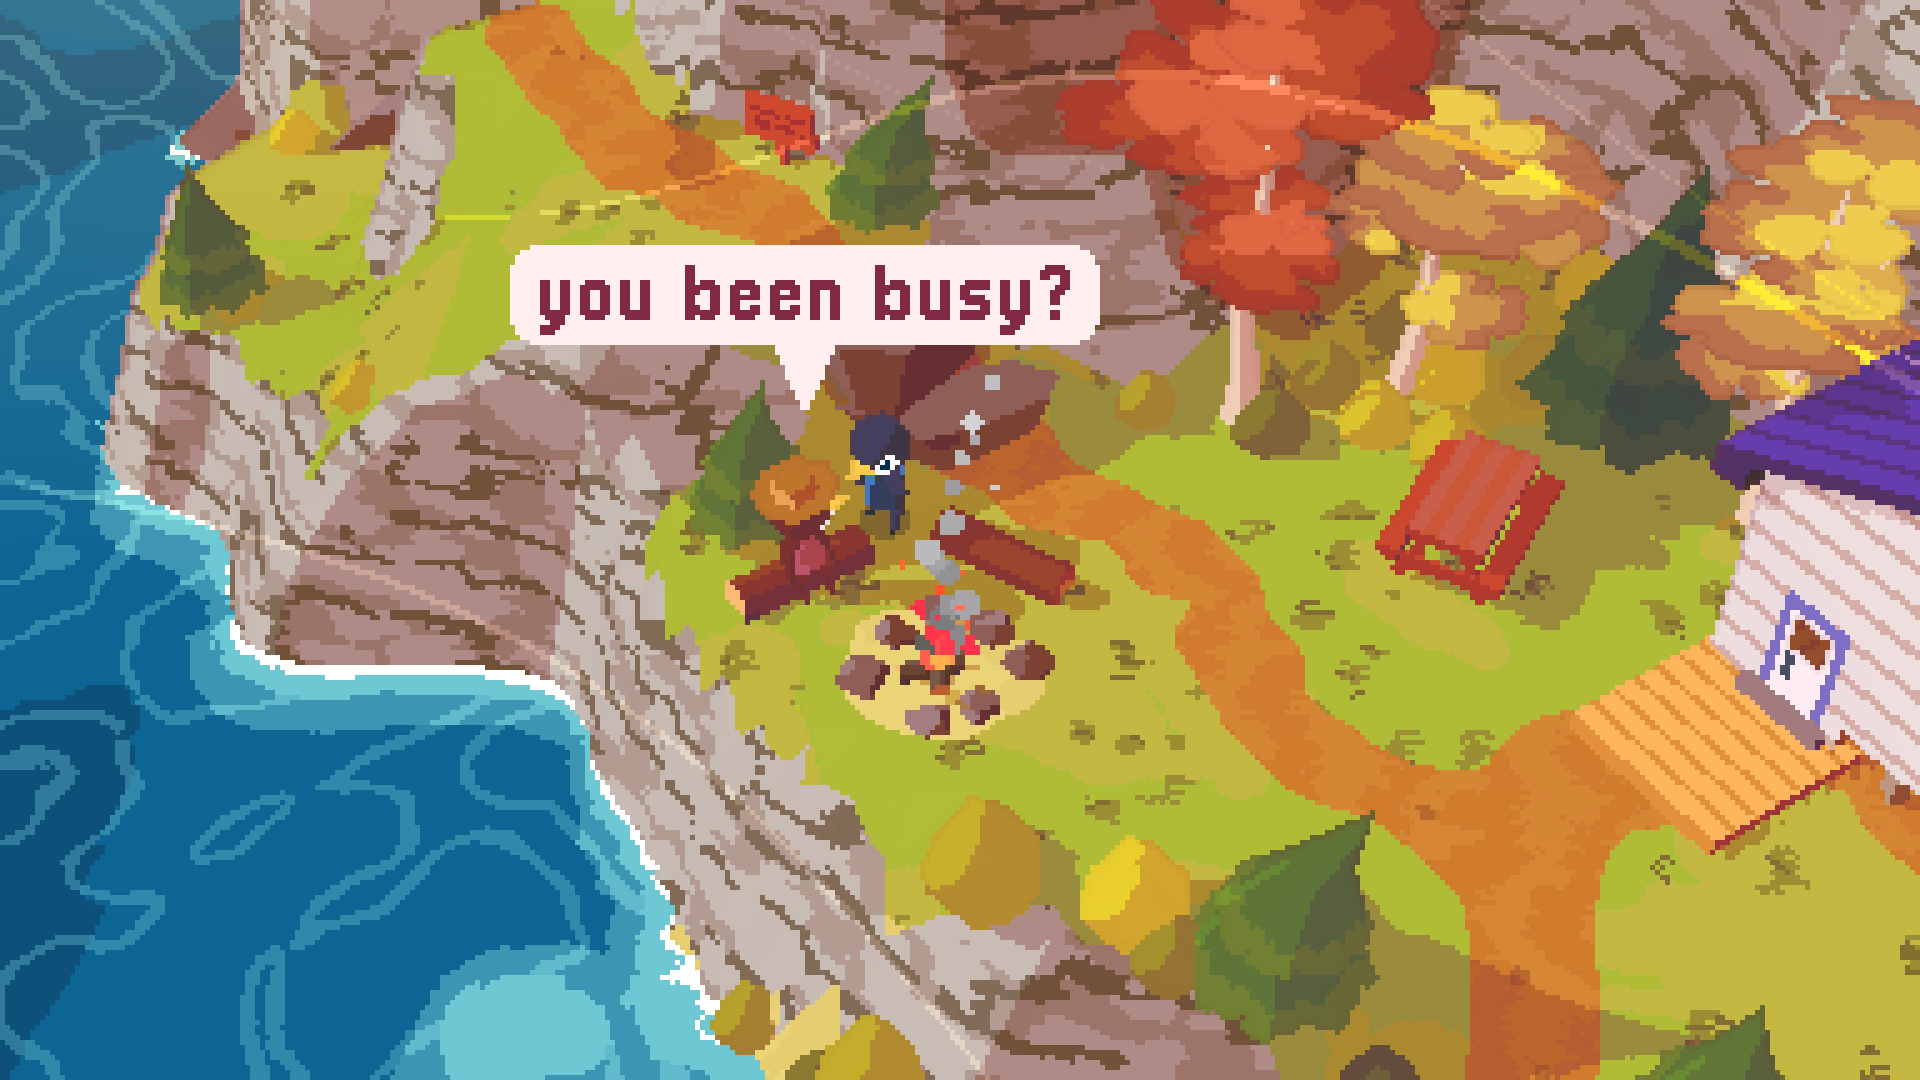
\includegraphics[width = 0.5\textwidth]{Imagenes/OCR/Pixel.png}
		\caption{Ejemplo imagen PixelArt }
		\label{fig:Pixelart}
	\end{figure}
	\item Texto en bocadillos(TxtBoc)(Figura \ref{fig:TxTBoc}). Imágenes donde el texto a reconocer se situa en un bocadillo y que el color del bocadillo tiene un alto contraste con el fondo.
	\begin{figure}[H]
		\centering
		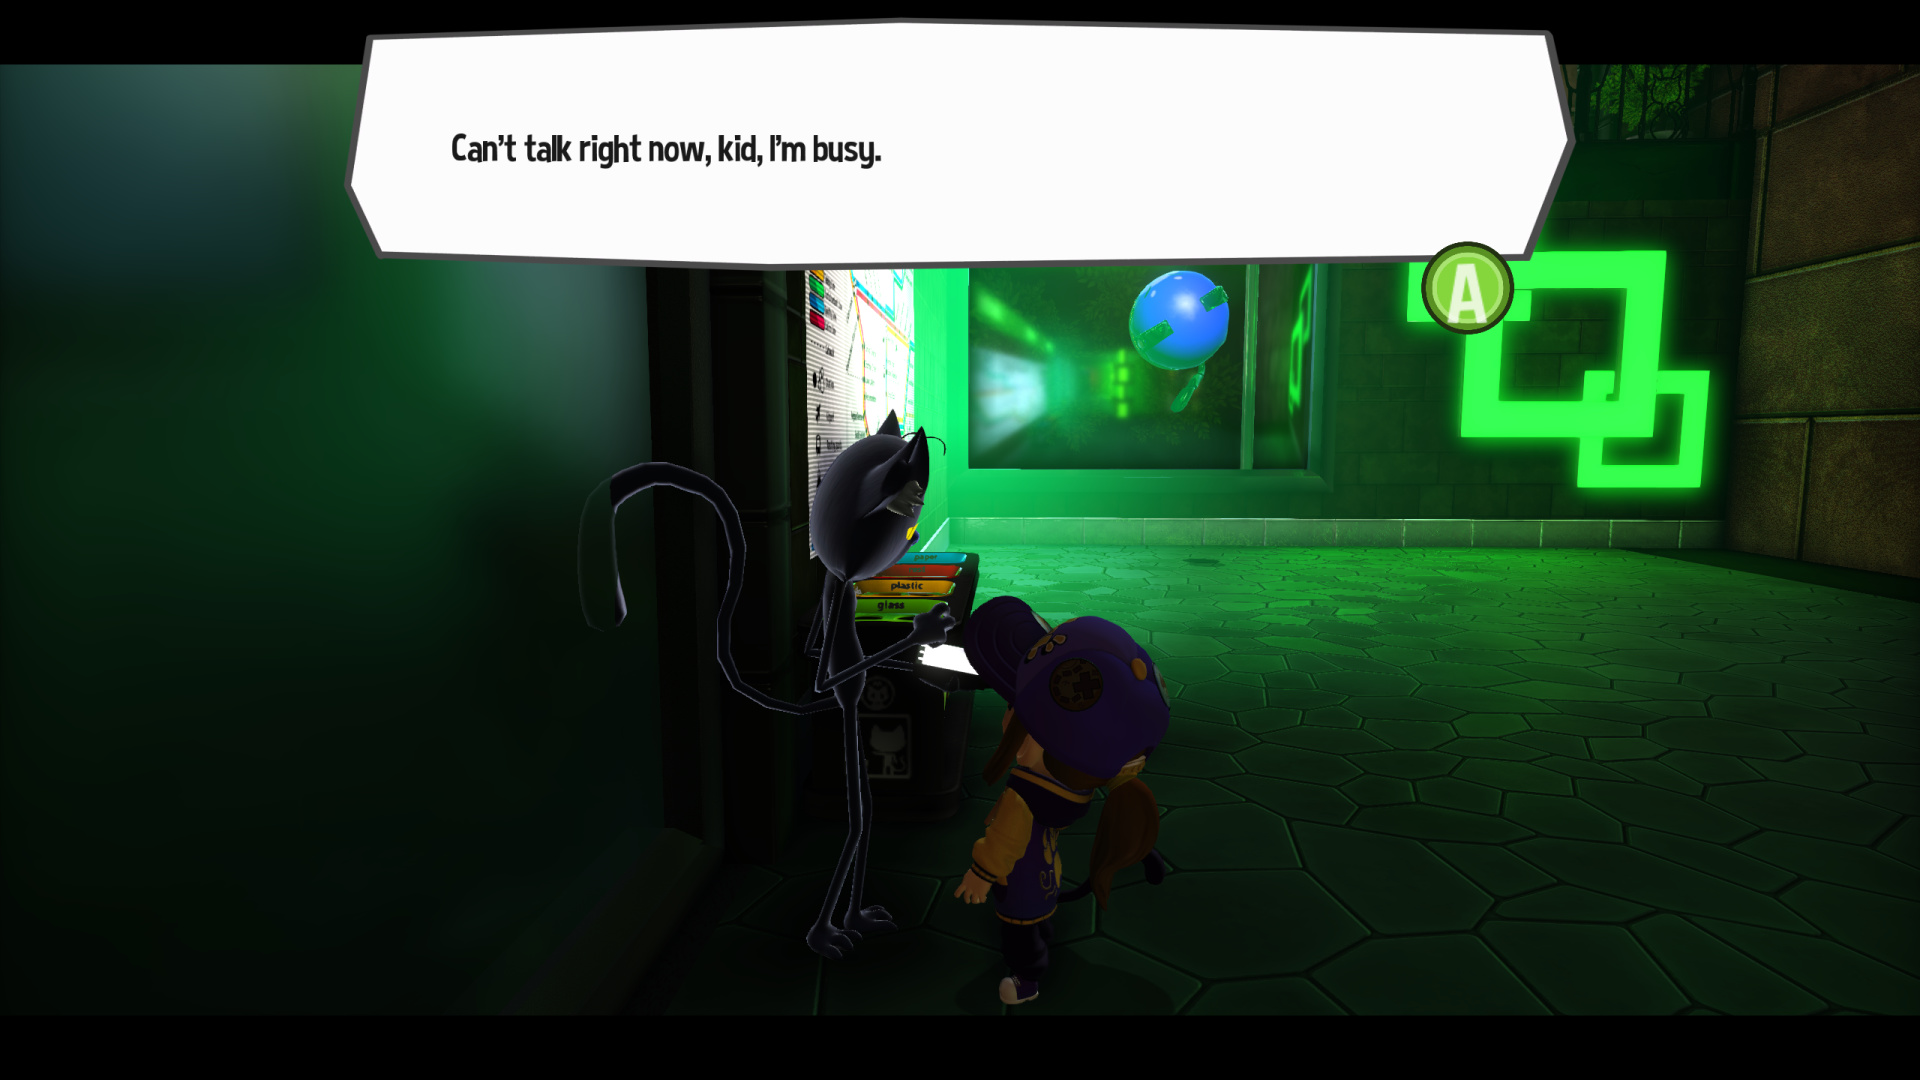
\includegraphics[width = 0.5\textwidth]{Imagenes/OCR/Boc.png}
		\caption{Ejemplo imagen de texto en bocadillo }
		\label{fig:TxTBoc}
	\end{figure}
	\item Texto en bocadillos con poca diferenciación con el fondo(TxtBoc2)(Figura \ref{fig:TxtBoc2}).Imágenes donde el texto a reconocer se situa en un bocadillo y que el color del bocadillo tiene un contraste medio o bajo con el fondo.
	\begin{figure}[H]
		\centering
		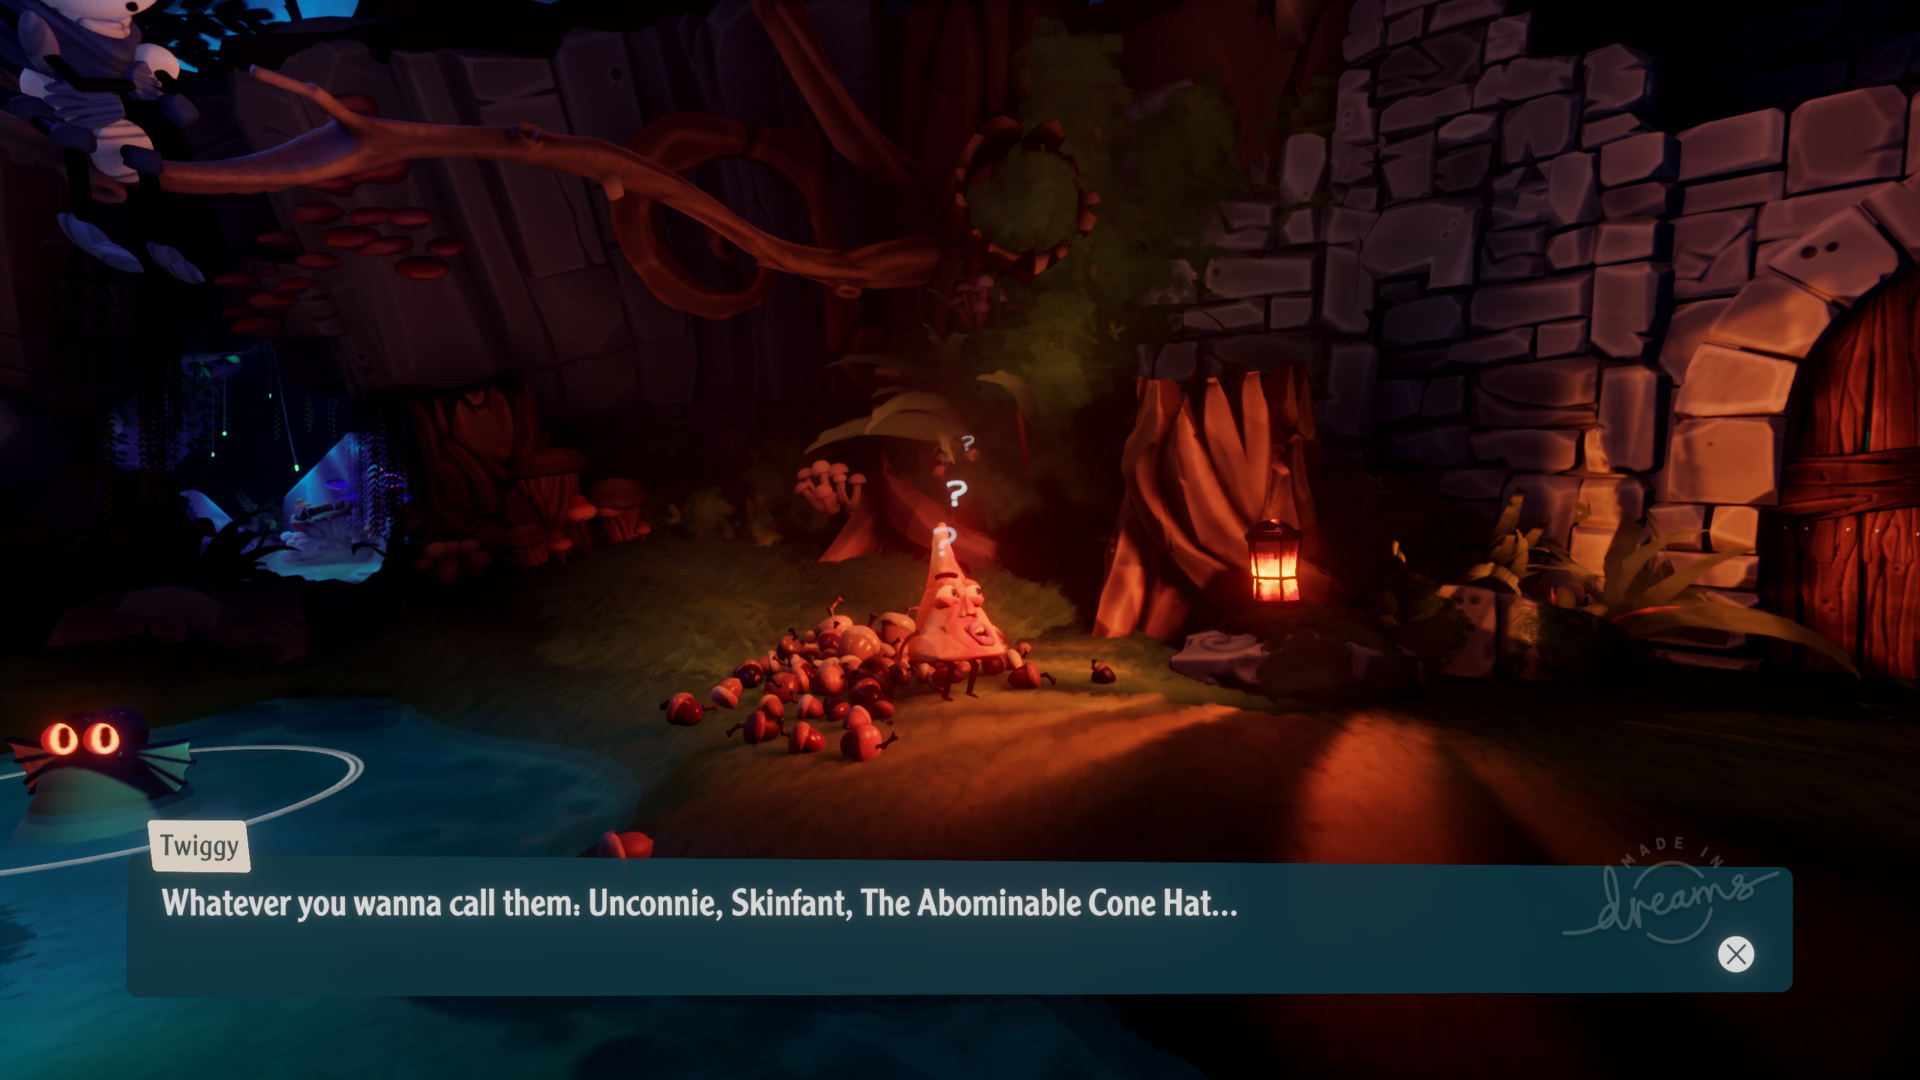
\includegraphics[width = 0.5\textwidth]{Imagenes/OCR/Boc2.png}
		\caption{Ejemplo imagen de texto en bocadillos con poca diferenciación con el fondo }
		\label{fig:TxtBoc2}
	\end{figure}
\end{enumerate} 


El preprocesamiento de imágenes consiste en aplicar técnicas que modifican las imágenes para que sea más fácil de reconocer por una OCR el texto existente.
Para saber que técnicas mejoran el reconocimiento, se ha ido probando con cada una de ellas en el manual de \cite{OpenCVProcessing}, obteniendo los resultados e identificando aquellas técnicas que ayuda a mejorar el CER medio.
Las técnicas probadas son las siguientes:

\begin{enumerate}
	\item Escala de grises(Figura \ref{fig:EscalaGrises}):
	Convierte una imagen a un formato de un solo canal, representando solo la intensidad de luz. Es útil para simplificar y reducir la cantidad de datos cuando el color no es relevante.
	\begin{figure}[H]
		\centering
		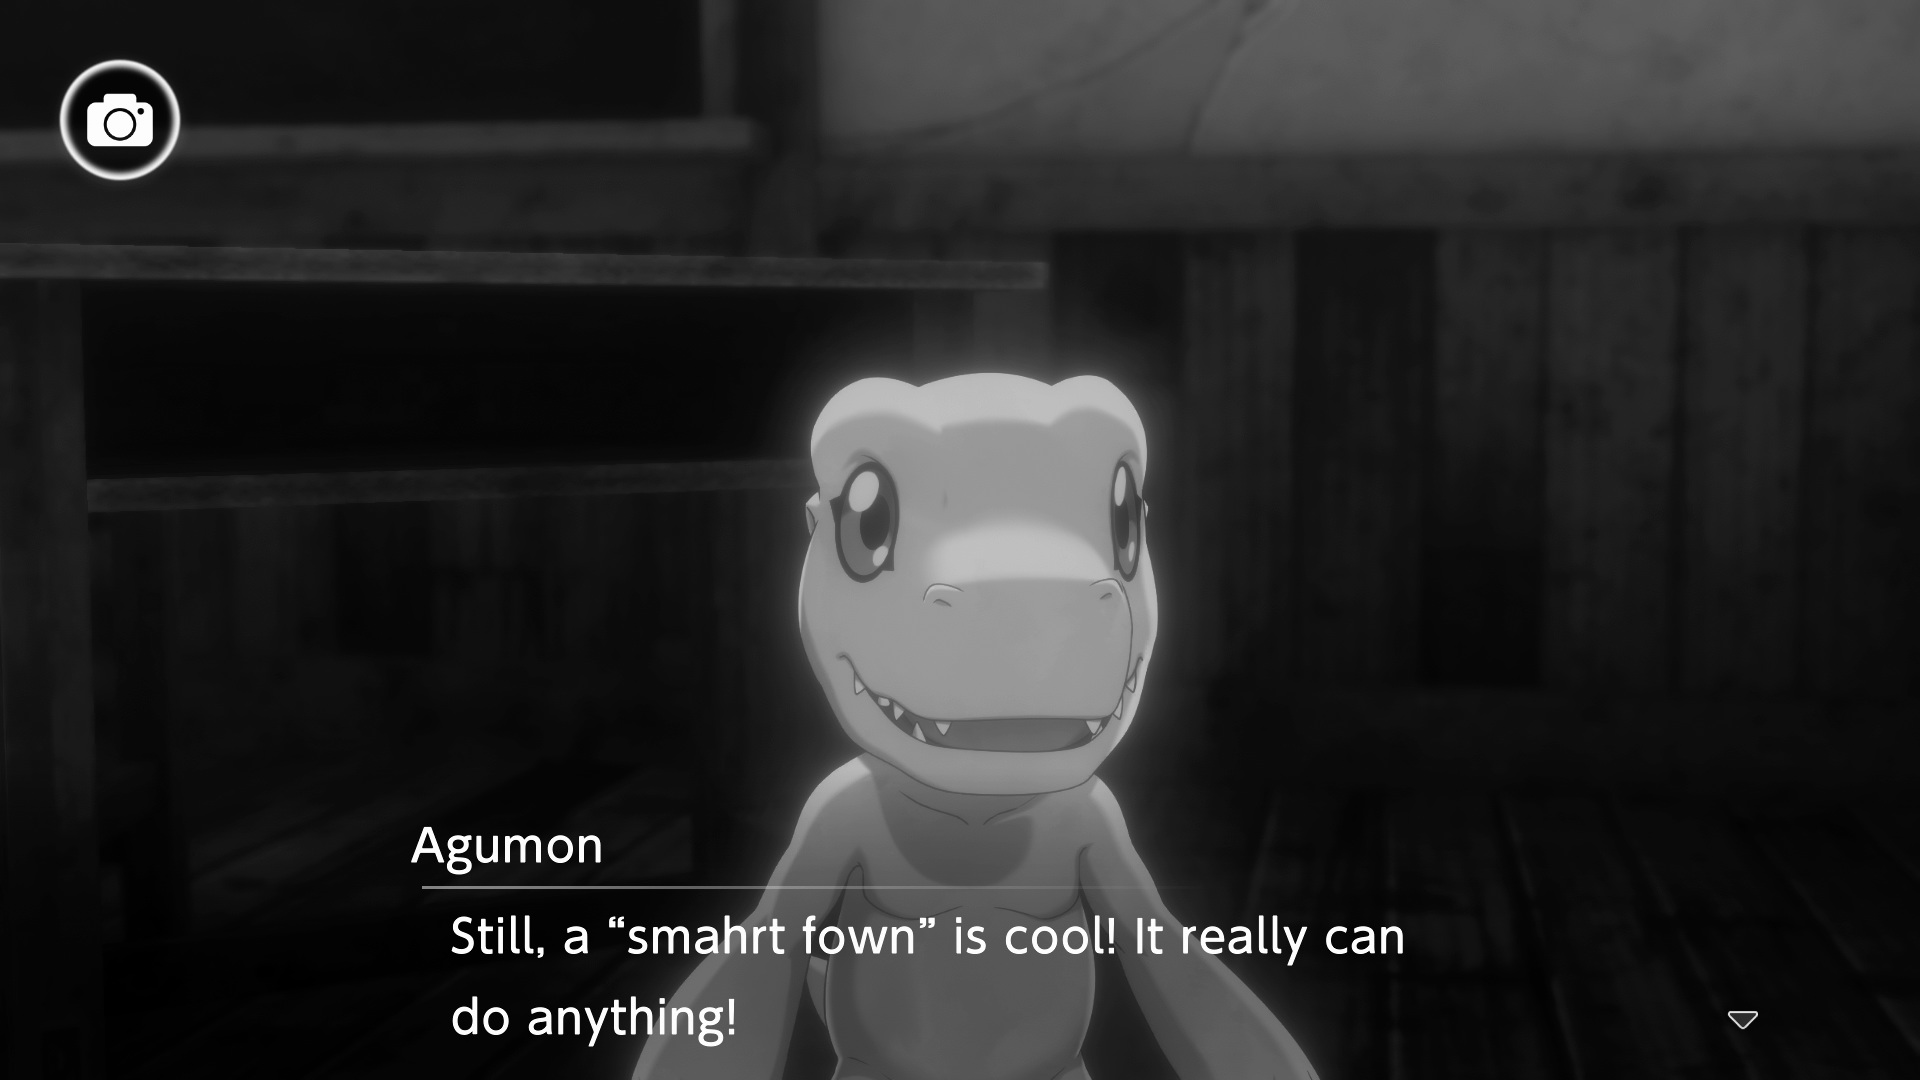
\includegraphics[width = 0.5\textwidth]{Imagenes/Preprocesado/1.png}
		\caption{Imagen a escala de grises}
		\label{fig:EscalaGrises}
	\end{figure}
	\item Aumentar contraste(Figura \ref{fig:Contraste}): 
	Mejora la diferencia entre las áreas claras y oscuras en una imagen, lo que facilita la detección de detalles.
	\begin{figure}[H]
		\centering
		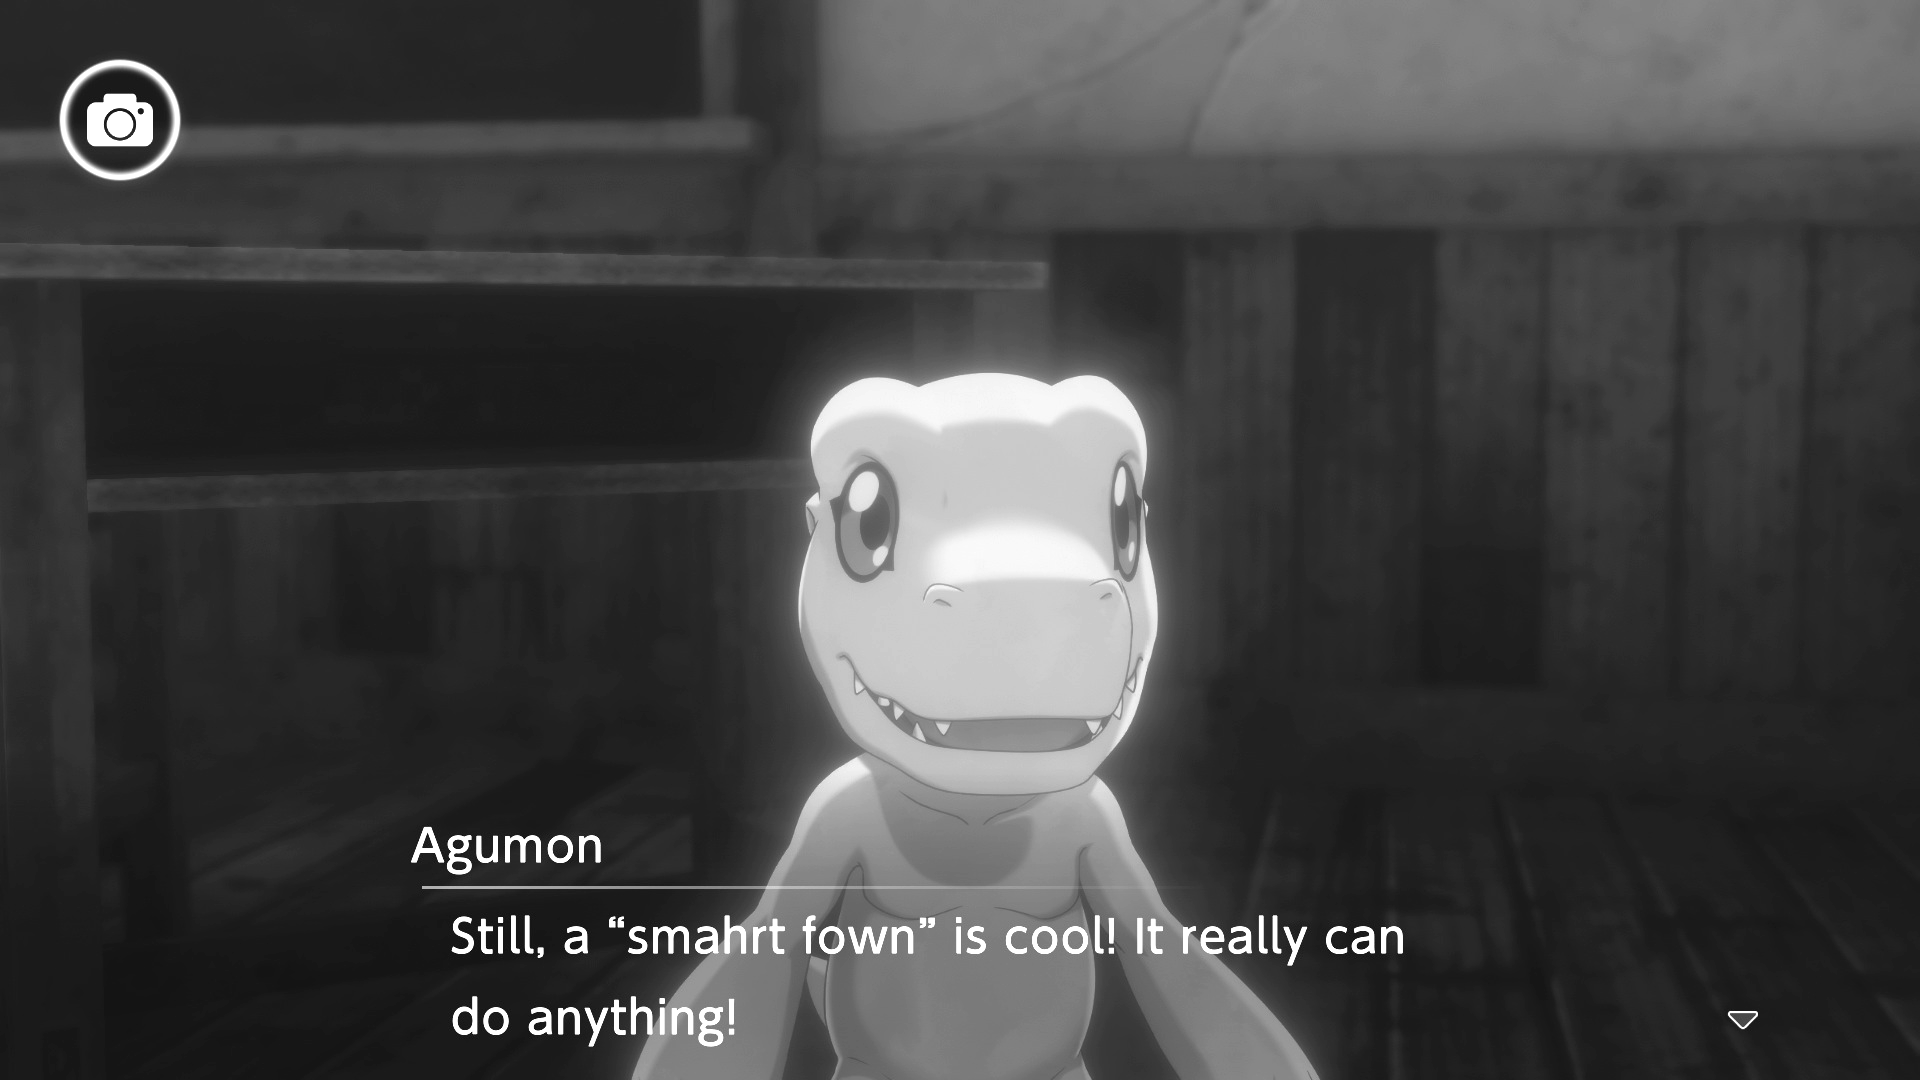
\includegraphics[width = 0.5\textwidth]{Imagenes/Preprocesado/2.png}
		\caption{Imagen con aumento de contraste}
		\label{fig:Contraste}
	\end{figure}
	\item Ecualización del histograma(Figura \ref{fig:Histograma}):
	Ajusta el contraste de la imagen extendiendo la distribución de los niveles de gris, mejorando el rango dinámico y resaltando los detalles.
	\begin{figure}[H]
		\centering
		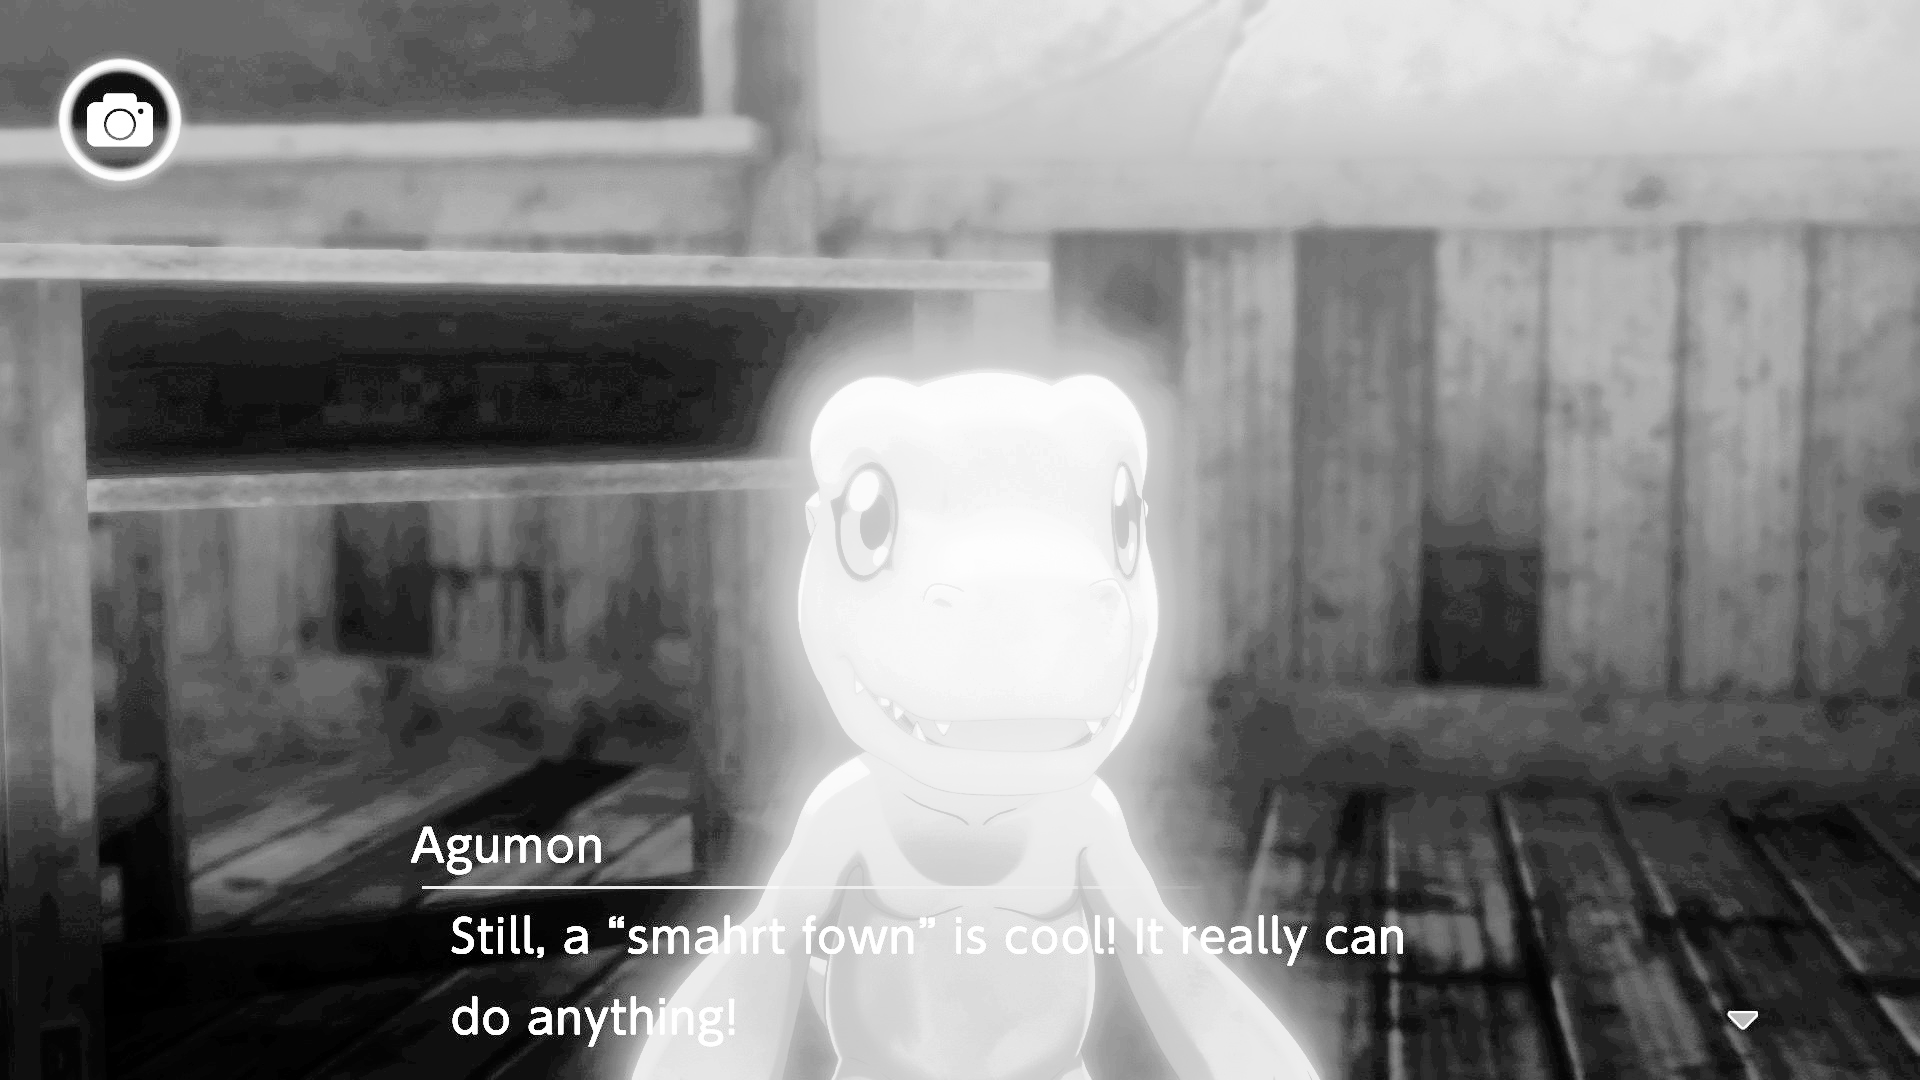
\includegraphics[width = 0.5\textwidth]{Imagenes/Preprocesado/3.png}
		\caption{Imagen con ecualización de histograma}
		\label{fig:Histograma}
	\end{figure}
	
	\item Corrección del gamma(Figura \ref{fig:Gamma}):
	Ajusta los valores de intensidad en la imagen para compensar la percepción humana y los errores del sensor, lo que puede hacer que ciertas áreas sean más visibles.
	\begin{figure}[H]
		\centering
		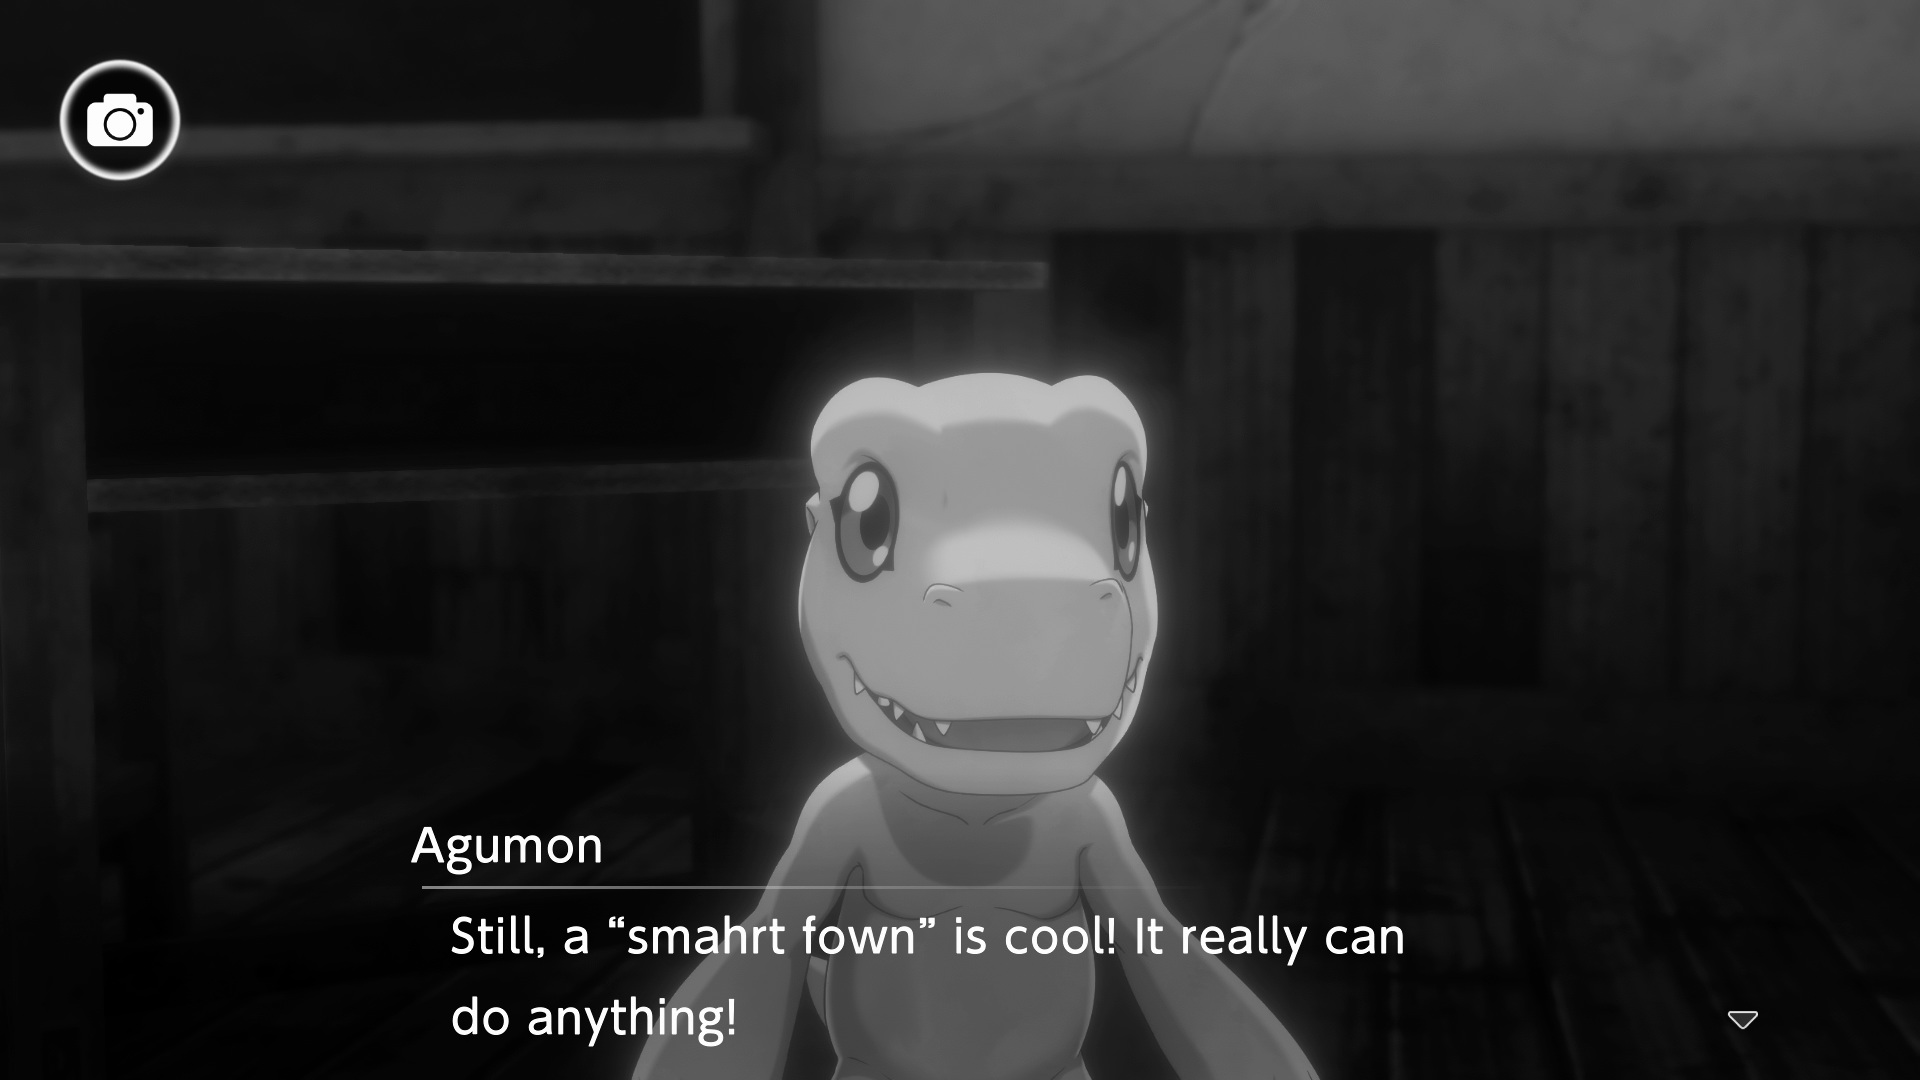
\includegraphics[width = 0.5\textwidth]{Imagenes/Preprocesado/4.png}
		\caption{Imagen con corrección del gamma}
		\label{fig:Gamma}
	\end{figure}
	
	\item Filtro de nitidez(Figura \ref{fig:F.Nitidez}): 
	Realza los bordes de una imagen para destacar detalles, útil en aplicaciones donde se requiere mayor definición.
	\begin{figure}[H]
		\centering
		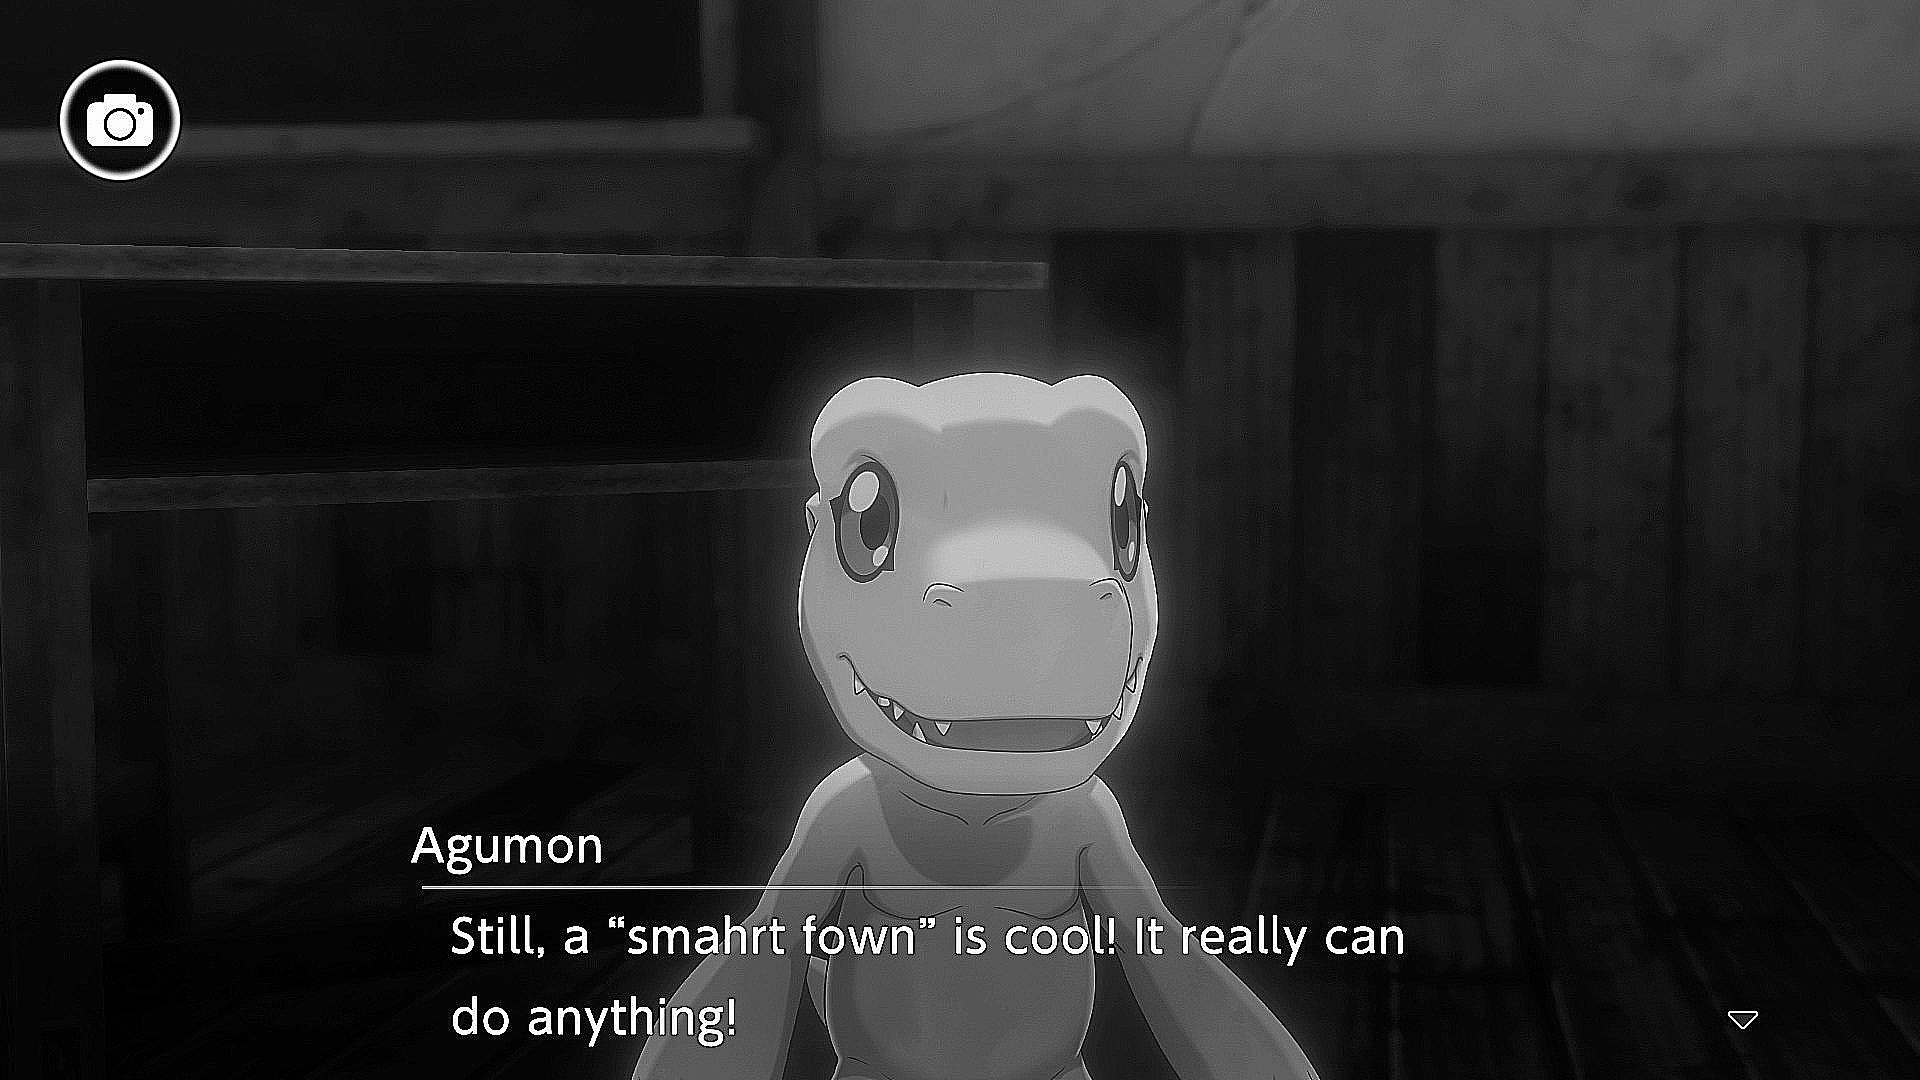
\includegraphics[width = 0.5\textwidth]{Imagenes/Preprocesado/5.png}
		\caption{Imagen con filtro de nitidez}
		\label{fig:F.Nitidez}
	\end{figure}
	
	\item Adaptive Thresholding(Figura \ref{fig:Thresholding}):
	Segmenta una imagen dividiéndola en áreas claras y oscuras, aplicando un umbral que se ajusta de forma adaptativa a las variaciones locales de luz.
	\begin{figure}[H]
		\centering
		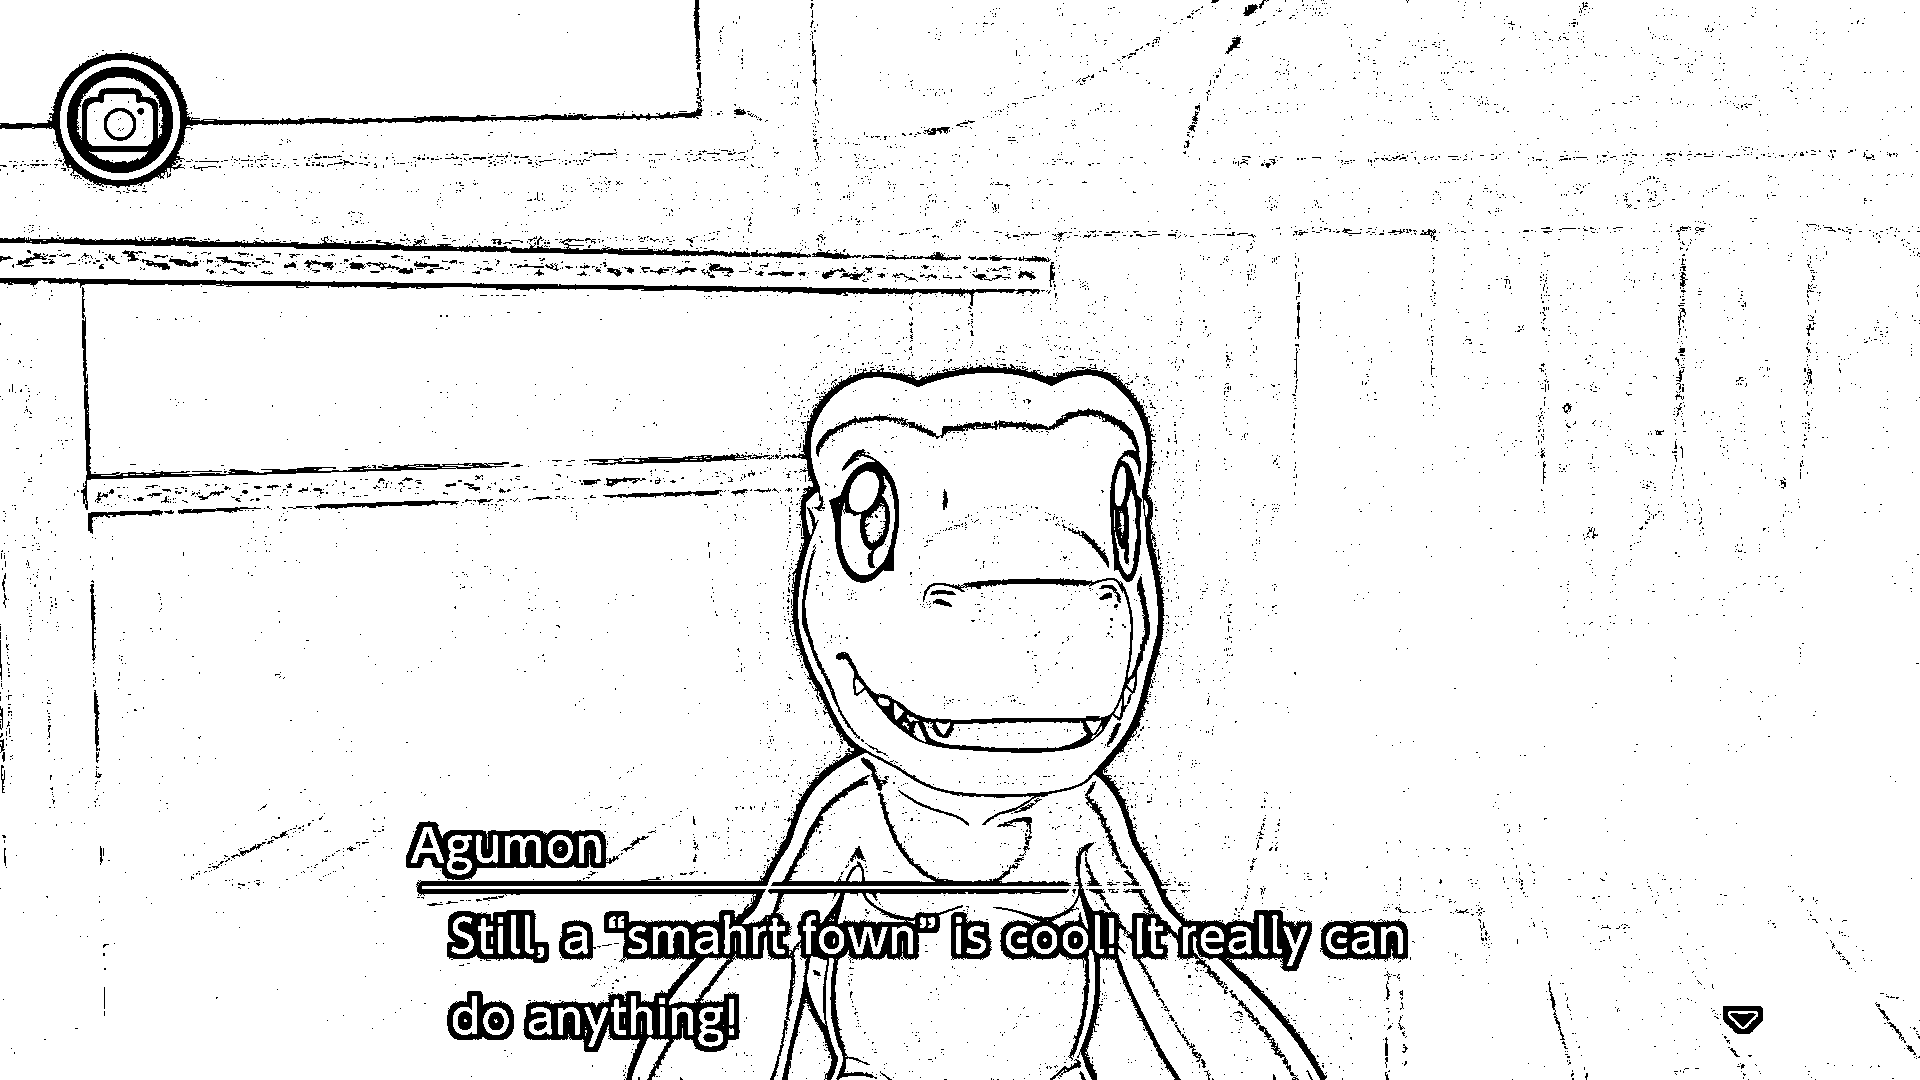
\includegraphics[width = 0.5\textwidth]{Imagenes/Preprocesado/6.png}
		\caption{Imagen aplicando adaptive thresholding}
		\label{fig:Thresholding}
	\end{figure}
	
	\item Simple Thresholding(Figura \ref{fig:S.Threshold}): 
	Asigna un valor binario a cada píxel dependiendo de si está por encima o por debajo de un umbral específico, útil para crear máscaras y segmentación sencilla.
	\begin{figure}[H]
		\centering
		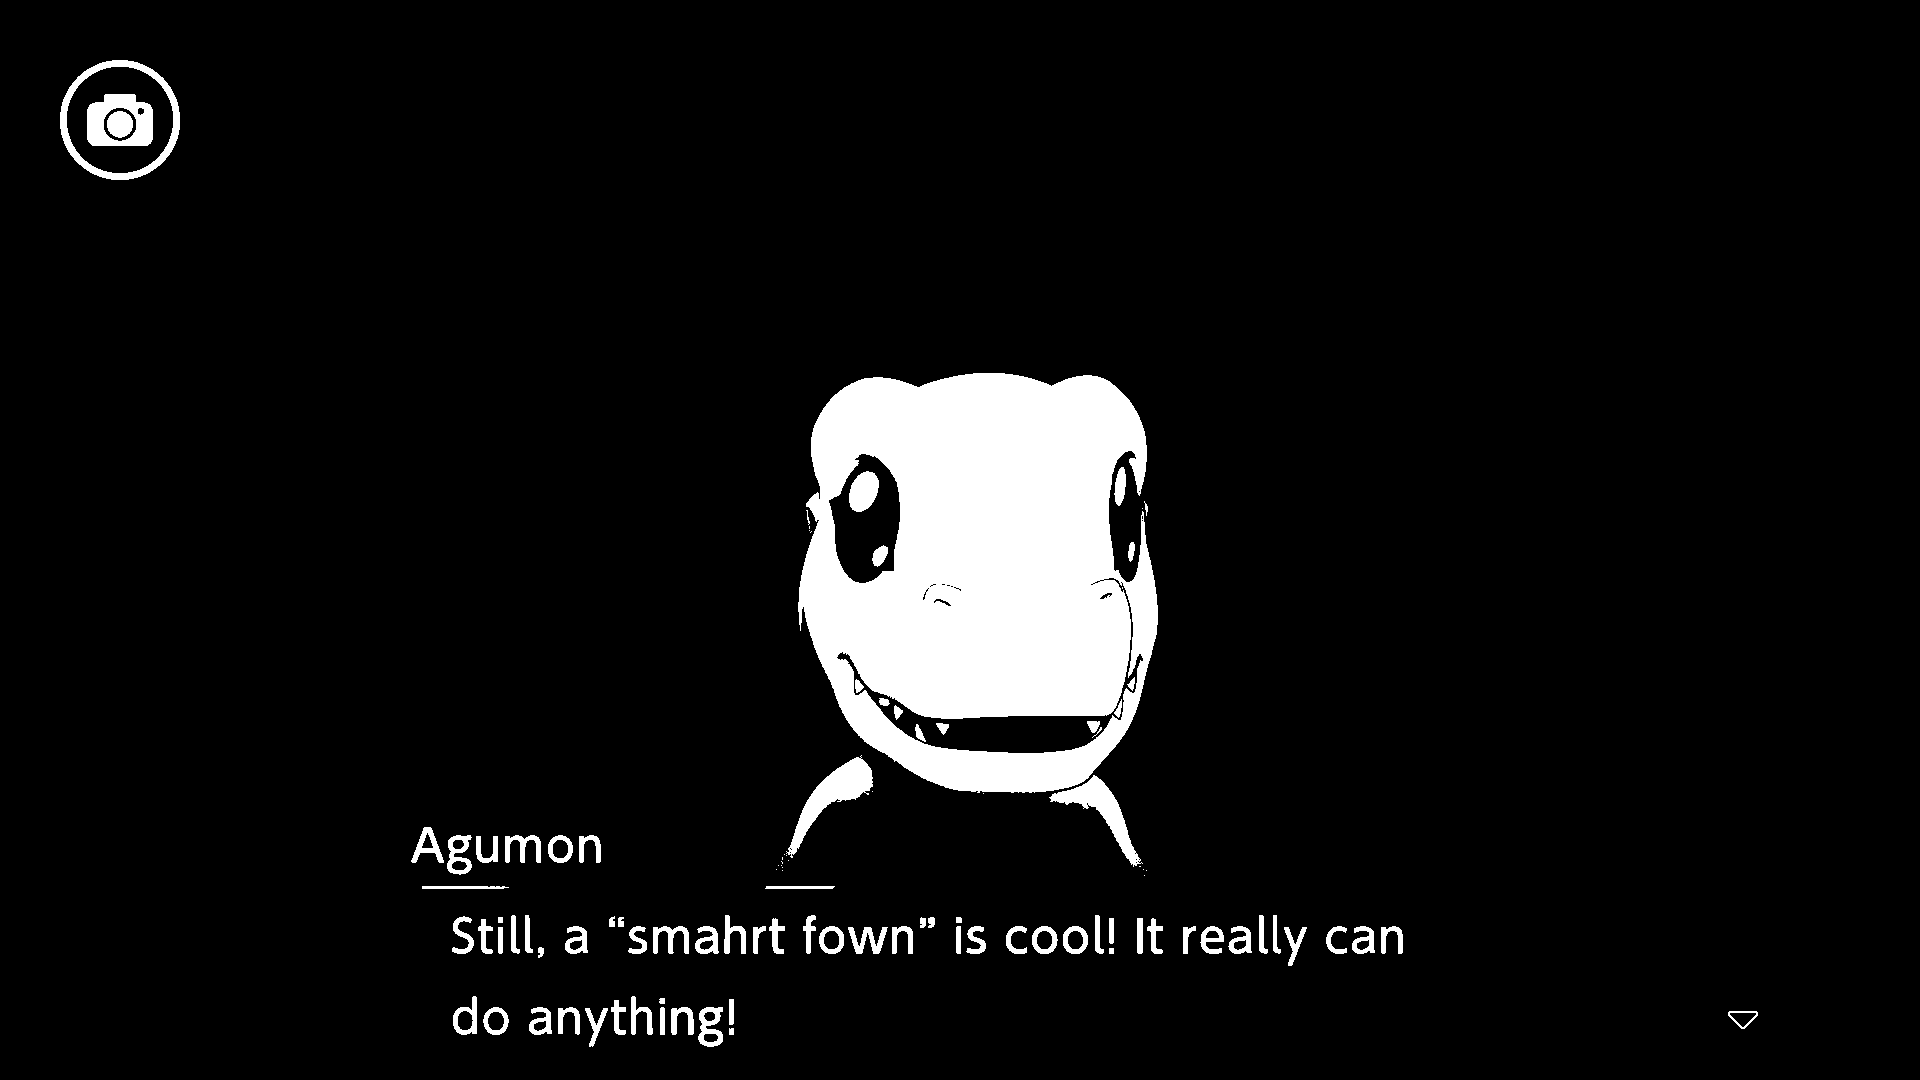
\includegraphics[width = 0.5\textwidth]{Imagenes/Preprocesado/7.png}
		\caption{Imagen aplicando simple thresholding}
		\label{fig:S.Threshold}
	\end{figure}
	
	\item Image Blurring (Desenfoque de Imagen)(Figura \ref{fig:Blurring}): 
	Reduce el ruido y los detalles mediante técnicas como filtros Gaussianos o de promediado, comúnmente utilizado para suavizar imágenes antes de un análisis.
	\begin{figure}[H]
		\centering
		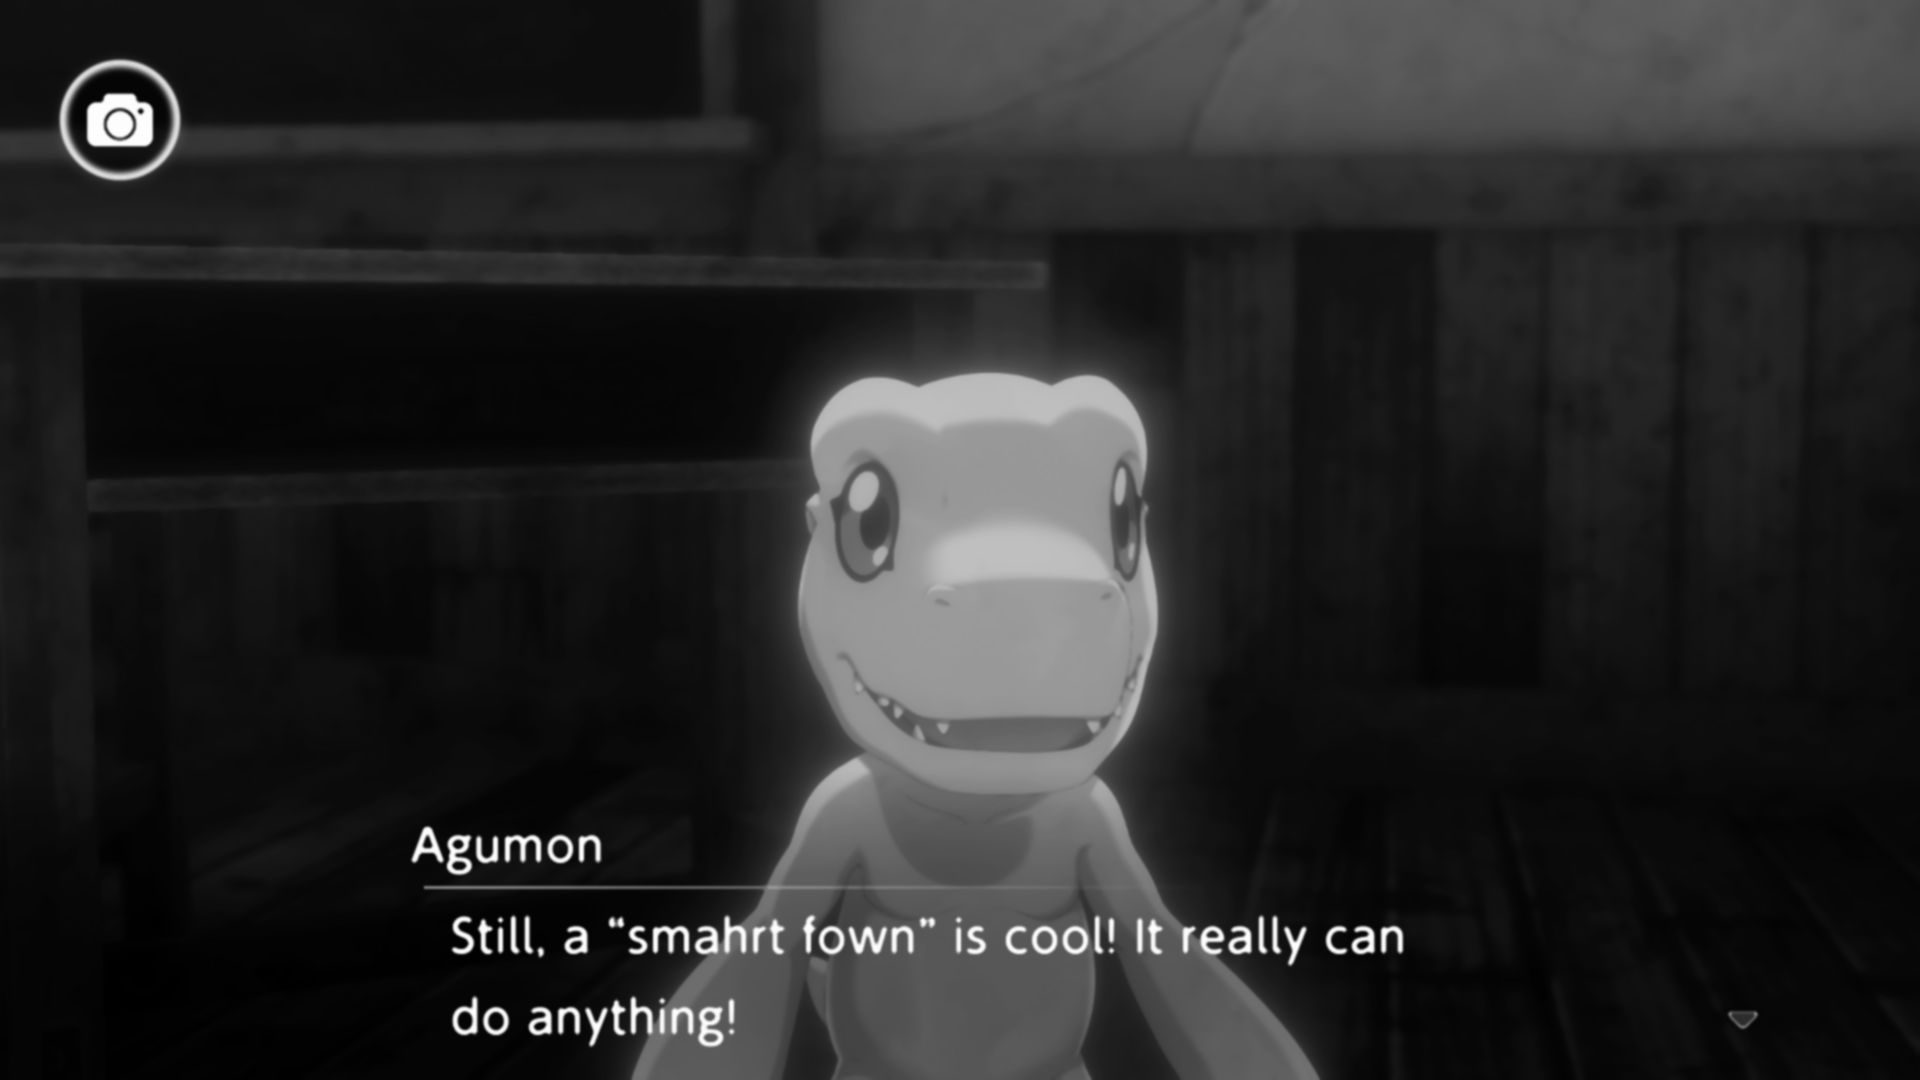
\includegraphics[width = 0.5\textwidth]{Imagenes/Preprocesado/8.png}
		\caption{Imagen aplicando desenfoque de imagen}
		\label{fig:Blurring}
	\end{figure}
	
	\item Redimensionar la imagen: 
	Cambia las dimensiones de una imagen, lo que puede ser útil para normalizar entradas a una red neuronal o ajustar el tamaño de una imagen para procesamiento.
	
	\item Dilatar y erosionar(Figura \ref{fig:Dilate_Erode}): 
	Técnicas de morfología matemática que expanden o reducen las regiones blancas (o los objetos) en una imagen binaria, útiles para limpieza de ruido o cierre de contornos.
	\begin{figure}[H]
		\centering
		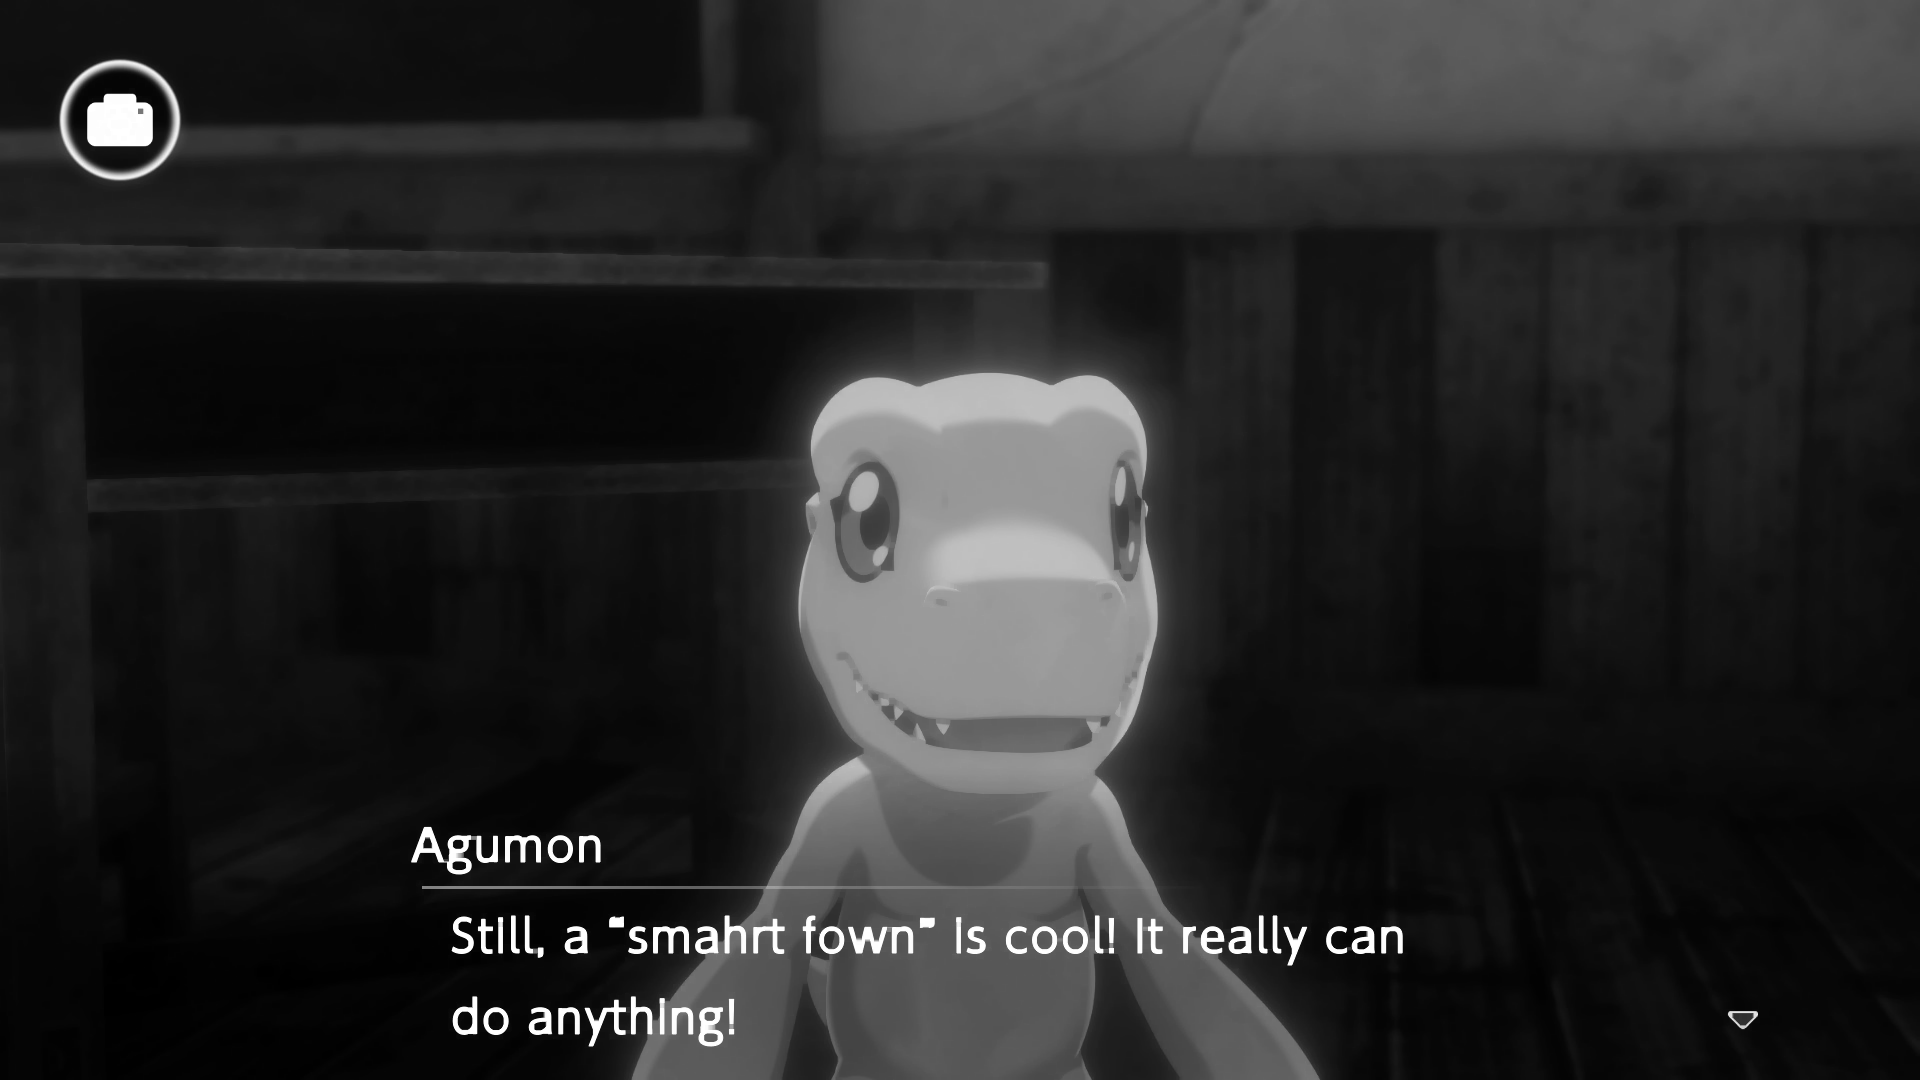
\includegraphics[width = 0.5\textwidth]{Imagenes/Preprocesado/10.png}
		\caption{Imagen dilatado y erosionado}
		\label{fig:Dilate_Erode}
	\end{figure}
	
	\item Denoising (Reducción de ruido)(Figura \ref{fig:Denoising}): 
	Elimina o reduce el ruido en una imagen para mejorar la calidad visual y el rendimiento de tareas de reconocimiento.
	\begin{figure}[H]
		\centering
		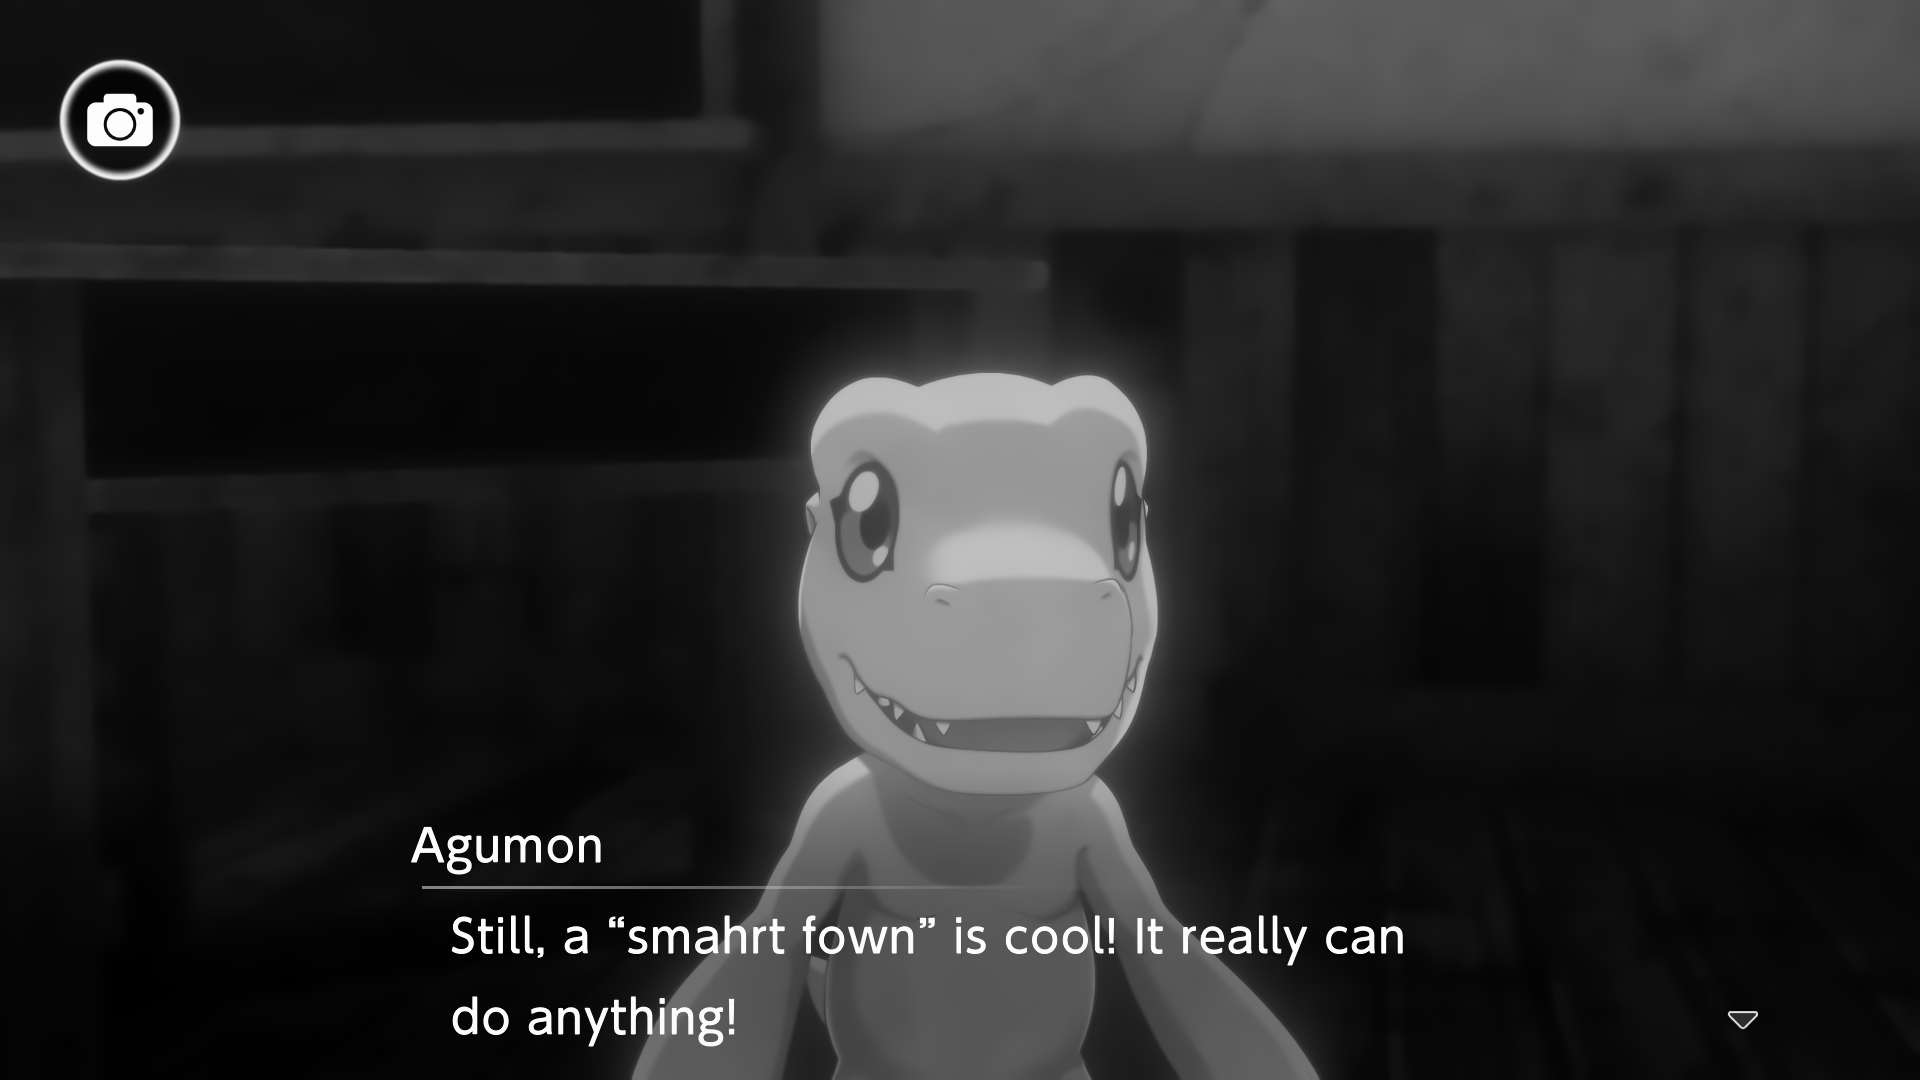
\includegraphics[width = 0.5\textwidth]{Imagenes/Preprocesado/11.png}
		\caption{Imagen aplicando reducción de ruido}
		\label{fig:Denoising}
	\end{figure}
	\begin{table}[H]
		\begin{tabular}{llllll}
			Tipo                                                                 & F.Complejo                      & F.Simple                      & PixelArt                      & TxTBoc                       & TxtBoc2                       \\
			Nada                                                               & 9.39                          & 1.05                         & 2.51                          & 2.02                         & 5.61                          \\
			Grises                                                               & 3.72                          & 0.59                         & 2.69                          & 1.17                         & 2.16                          \\
			Contraste                                                            & 5.06                          & 0.81                         & 2.39                          & 1.13                         & 10.07                         \\
			\begin{tabular}[c]{@{}l@{}}Ecualización\\ de histograma\end{tabular} & 5.59                          & 3.60                         & 6.56                          & 2.41                         & 8.67                          \\
			Gamma                                                                & 3.72                          & 0.59                         & 2.69                          & 1.17                         & 2.16                          \\
			Filtro de nitidez                                                    & 11.06                         & 2.17                         & 8.84                          & 3.29                         & 12.05                         \\
			Thresholding C                                                       & \cellcolor[HTML]{FF0000}16.80 & \cellcolor[HTML]{FF0000}9.44 & 10.36                         & 4.08                         & \cellcolor[HTML]{FF0000}23.44 \\
			\begin{tabular}[c]{@{}l@{}}Thresholding\\ Gaussian\end{tabular}      & 12.85                         & 9.35                         & \cellcolor[HTML]{FF0000}16.16 & \cellcolor[HTML]{FF0000}4.71 & 22.83                         \\
			Thresold Binary                                                      & 4.05                          & \cellcolor[HTML]{00FF00}0.49 & 2.14                          & 1.79                         & 2.04                          \\
			\begin{tabular}[c]{@{}l@{}}Redimension\\ x1.5\end{tabular}           & 4.77                          & 0.80                         & 2.86                          & 1.27                         & 3.07                          \\
			Gaussian Blur                                                        & 3.02                          & 0.68                         & 2.34                          & 1.14                         & 1.86                          \\
			Median Blur                                                          & 2.75                          & 0.51                         & 2.75                          & 1.25                         & 1.37                          \\
			2 Blur                                                               & 2.26                          & 0.59                         & 2.15                          & 1.22                         & \cellcolor[HTML]{00FF00}1.09  \\
			Dilatación y erosión                                                 & 2.19                          & 0.51                         & 2.48                          & \cellcolor[HTML]{00FF00}0.69 & 1.83                          \\
			Dilatación                                                           & \cellcolor[HTML]{00FF00}1.80  & 0.62                         & \cellcolor[HTML]{00FF00}1.23  & 0.80                         & 5.53                          \\
			Erosión                                                              & 2.02                          & 1.00                         & 2.57                          & 0.82                         & 1.21                          \\
			Denoising                                                            & 3.23                          & 0.57                         & 2.64                          & 1.07                         & 1.70                         
		\end{tabular}
		\caption{Tabla con los resultados de CER medio de cada categoría de imágenes después de aplicar un tipo de preprocesamiento.}
		\label{table:preproCERtable}
	\end{table}
\end{enumerate}
A continuación se ha hecho el experimento de aplicar un solo tipo de preprocesamiento a todas las imágenes de cada categoría, ejecutando el OCR sobre las imágenes preprocesadas y obteniendo el CER de cada imágen y el CER medio de cada categoría. Este proceso se ha aplicado para cada uno de las posibles técnicas de preprocesamiento obteniendo el resultado en la tabla \ref{table:preproCERtable}. Cada columna representa la categoría de la imagen y cada fila representa el preprocesamiento aplicado a las imágenes. En este caso no se hace distinción de OCR ya que preprocesamiento se aplica directamente en las imágenes antes de ser pasados a la OCR por lo que no importa la librería de OCR que se este usando.
Se marca en rojo aquel tipo de preprocesamiento que da peor resultado en la categoría y en verde, aquel que da mejor resultado.


Como podemos observar, en la mayoría de los preprocesamientos, los resultados mejoran en comparación con la de sin aplicar nada. Sin embargo, hay otros que empeoran, esto es debido a que el preprocesamiento ha marcado más las líneas y las geometrías por lo que el OCR reconozca más caracteres ``basura''. Esto no significa que el OCR vaya ir a peor, puede que reconozca mejor el texto esperado pero añadiendo más basura que antes, algo que intentaremos resolver en el siguiente apartado. 

Obteniendo esta tabla y viendo los resultados de imágenes se ha ido probando distintas combinaciones de preprocesados de imágenes:
\begin{enumerate}
	\item Experimento 1: 
	\begin{itemize}
		\item Grises \item Escalado\item Adaptive Threshold \item Denoising \item Blurring \item Dilate\_Erode    
	\end{itemize}
		\item Experimento 2: 
	\begin{itemize}
		\item Grises\item Escalado\item Denoising Blurring  \item Dilate\_Erode\item Ec. Histograma \item Gamma \item F.Nitidez           
	\end{itemize}
		\item Experimento 3: 
	\begin{itemize}
		\item Grises \item Escalado\item Simple Threshold \item Denoising \item Blurring \item F.Nitidez \item Dilate\_Erode    
	\end{itemize}
		\item Experimento 4: 
	\begin{itemize}
		\item Grises \item Escalado\item Simple Threshold \item Denoising \item Blurring \item Dilate\_Erode    
	\end{itemize}
\end{enumerate}
Obteniendo estos resultados:
\begin{table}[H]
	\begin{tabular}{llllll}
		Experimento & Complejo & Simple & PixelArt & TxTBoc & TxtBoc2                      \\
		 1 & 18.79     & 3.96   & 13.93     & 5.26   & 22.01 \\
		 2 & 7.23     & 4.58   & 14.96     & 4.94   & 11.94 \\
		 3 & 3.68     & 0.34   & 2.30     & 1.16   & 1.62 \\
		 4 & 2.57     & 0.29   & 2.01     & 1.01   & 1.49
	\end{tabular}
	\caption{Tabla con los resultados CER de cada categoría en cada experimento.}
	\label{table:Prepro}
\end{table}
Donde podemos ver en la tabla \ref{table:Prepro} que el experimento más destacado es el experimento 4, por lo que en adelante seguiremos el preprocesamiento con las técnicas del experimento 4.
\subsection{Eliminación de caracteres basura}
\label{subsec:Eliminación de caracter basura}
Obteniendo el resultado de CER medio de los preprocesamientos(tabla \ref{table:preproCERtable}), podemos ver que se produce muchos números que superan al 1, esto significa que el OCR ha reconocido más caracteres de lo que hay en el texto esperado, todos esos caracteres que sobran son caracteres basura y el texto que necesitaremos estará en algunas de esas líneas. En esta sección intentaremos eliminar esos caracteres basura dejando solo lo necesario.
\begin{figure}[H]
	\centering
	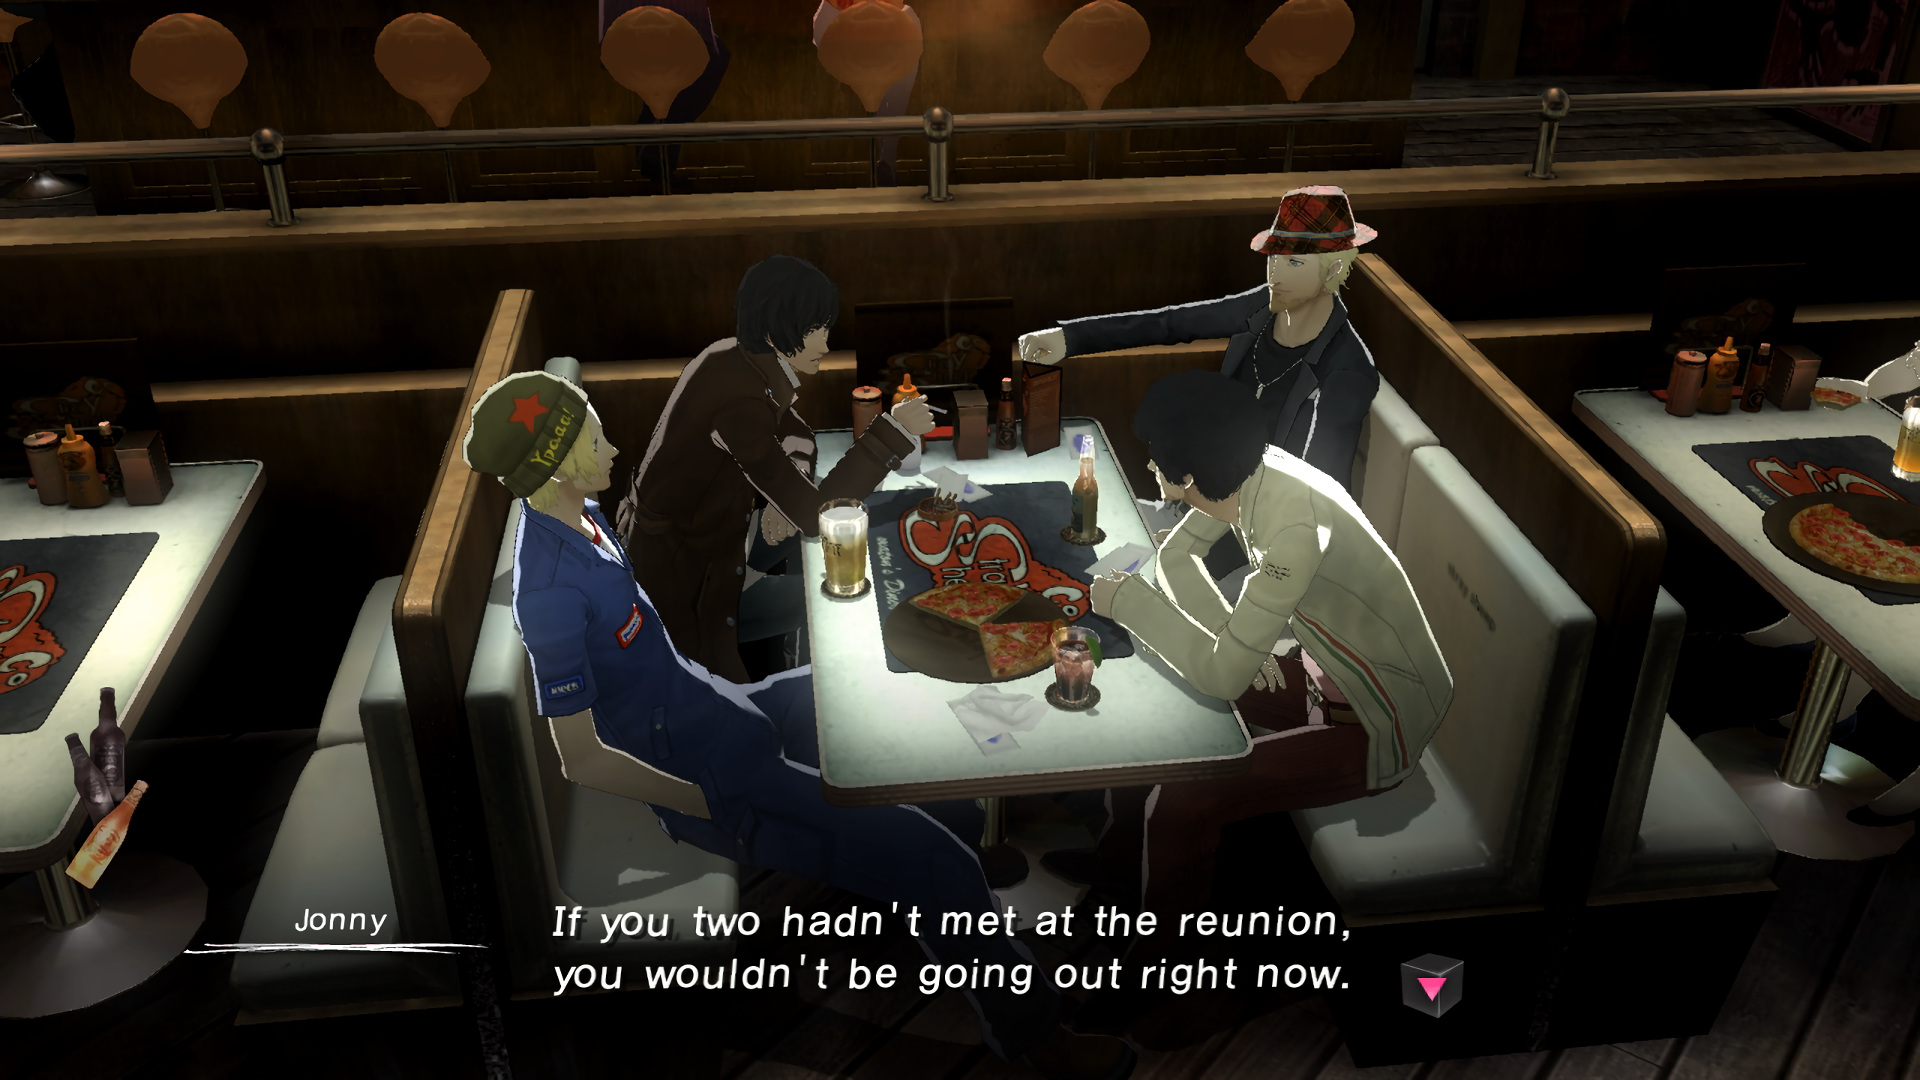
\includegraphics[width = 1\textwidth]{Imagenes/Sample_Trash_Char.png}
	\caption{Imagen ejemplo.}
	\label{fig:Trash_Char}
\end{figure}

El texto esperado de la figura \ref{fig:Trash_Char} es la siguiente:
\begin{verbatim}
	Jonny
	If you two hadn't met at the reunion,
	you wouldn't be going out right now.
\end{verbatim}
Y una posible salida de la OCR con la figura \ref{fig:Trash_Char} puede ser la siguiente:
\begin{verbatim}
T A W
Wml"lll"|||"lll“1]]“11‘“"1“l‘l]1"]]]"]]1"1V‘“"‘”V"”””””“WWHH\HH\HH
G
wiui:lfifl}m;,;r}l’“
Nul1l1lmu11111um111llumI11llumIIIIIIMMI1IllMmlllIIIUU1
Hunum;.x:flwww'M;‘dm‘w‘w‘w‘w‘uHfl“fl“flflmw e 4 ‘ w}\‘s.*"‘r Ll e e p
: L T Q1 A it e
- ' diiry el R ;4
o wm W el 5
i " :_.“;»"*‘ i i m?“ Q:‘]m}illl}jjw ! “hu‘11111111{}}“
T i 1‘11“1””“””““” HHHHHHH ‘HHU”“HH\HHHHH\HMH\H ‘ (TR
I e > h ¢ 4 ' i
= 4 o
T
- i e
§ ...
E ‘E | \ i
P S y:
,,|,- |
IR ill ‘
— ' A 000 Ir yo
\end{verbatim}

Donde de forma subjetiva no encontramos ningún trozo del texto que se corresponda o sea parecido al ground-truth.

Después de aplicar el preprocesamiento elegido en el apartado anterior obtenemos el siguiente resultado:

\begin{verbatim}
T A W
Wml"lll"|||"lll“1]]“11‘“"1“l‘l]1"]]]"]]1"1V‘“"‘”V"”””””“WWHH\H
dJonny If you two hadn't met at the reunion 
you wouldn't be going out right now
,,|,- |
IR ill ‘
— ' A 000 Ir yo
\end{verbatim}

En esta salida ya podemos reconocer que hay dos líneas que se corresponde con la salida que esperamos.
La frase que realmente importa es solamente las dos líneas de la salida.
\begin{verbatim}
Jonny If you two hadn't met at the reunion
you wouldn't be going out right now
\end{verbatim}
Esto es un problema importante que debemos solucionar ya que es imposible saber si un test es correcto o no con esta entrada.

En esta sección se propone una solución a este problema de caracteres ``basura'' usando el algoritmo de distancia \emph{levenshtein}.

La distancia de Levenshtein(también conocida como distancia de edición) según un articulo de \cite{LevDistance} se define como una métrica que mide el número mínimo de operaciones necesarias para transformar una cadena en otra, utilizando tres tipos de operaciones básicas:
\begin{itemize}
\item Inserciones: Agregar un carácter.
\item Eliminaciones: Eliminar un carácter.
\item Sustituciones: Reemplazar un carácter por otro.
\end{itemize}


Suponiendo que tenemos el texto esperado de la imagen,  utilizando esta métrica, podemos obtener la distancia levenshtein entre una línea del texto esperado y una línea del texto reconocido por la OCR. Con la distancia obtenida podemos calcular la similitud de las cadenas y aplicando un cierto umbral, podemos identificar aquellas líneas que más se asimila al texto esperado, obteniendo así las líneas deseadas y descartando aquellas que no cumpla un cierto umbral.

La fórmula general para calcular la similitud es:

$Simulitud = 1-\frac{d}{max(s1,s2)} $ 

Donde:

\textit{d} es la distancia levenshtein.

\textit{max(s1,s2)}	 es el máximo entre la longitud de la cadena \textit{s1} y cadena \textit{s2}

Uno de los resultados obtenidos aplicando la distancia levenshtein es la siguiente si aplicamos un umbral de similitud de 0.8 (tiene que ser 80\% de parecido):
\begin{itemize}
\item Texto real de OCR:
\begin{verbatim}
"
|
\ J
—
Agumon /
Still, a “smahrt fown” is cool! It really can
do anything! <
\end{verbatim}
\item Texto esperado:
\begin{verbatim}
Agumon
Still,a "smahrt fown" is cool! It really can
do anything!
\end{verbatim}

El algoritmo de limpieza sigue los siguientes pasos:

\begin{enumerate}
	\item Se compara la primera línea obtenida por el OCR con la primera línea del texto esperado.
	\item Se calcula la distancia de Levenshtein entre ambas cadenas.
	\item A partir de la distancia de Levenshtein y la longitud de las cadenas, se calcula el valor de similitud.
	\item Se verifica si la similitud supera el umbral previamente definido.
	\item Si la similitud es superior al umbral, se marca la línea como válida. En caso contrario, se continúa con la siguiente línea del texto esperado.
	\item Este proceso se repite hasta haber comparado la línea del OCR con todas las líneas del texto esperado. Si durante la iteración se encuentra una línea con una similitud mayor que la obtenida hasta el momento, se actualiza la línea marcada con esta nueva coincidencia.
	\item El mismo procedimiento se repite para la segunda línea del OCR y para el resto de líneas subsiguientes.
\end{enumerate}
Después de todo ese proceso obtenemos la cadena limpiada utilizando distancia levenshtein.
\item Tras aplicar este algoritmo, la cadena de OCR resultante será la siguiente:
\begin{verbatim}
Agumon /
Still "smahrt fown" is cool! It really can 
do anything! <
\end{verbatim}
\end{itemize}  
Aplicando el algoritmo a los resultados de todas las imágenes de cada categoría mencionadas en el apartado anterior después de aplicar preprocesamiento obtenemos estos nuevos resultados del CER medio de cada categoría:

\begin{table}[H]
\begin{tabular}{llllll}
Tipo        & Complejo & Simple & PixelArt & TxTBoc & TxtBoc2                      \\
OCR         & 2.57     & 0.29   & 2.01     & 1.01   & \cellcolor[HTML]{FFFFFF}1.49 \\
Levenshtein & 0.63     & 0.16   & 0.63     & 0.55   & 0.42                        
\end{tabular}
\end{table}
El resultado de OCR es el resultado que obtenemos con solamente aplicando el preprocesamiento del apartado anterior. Sobre esa salida, se aplica la distancia levenshtein para la eliminación de basura obteniendo los nuevos resultados. Podemos ver en los números que mejoran casi un 50\% en todas la categorías por lo que es una técnica viable para nuestra herramienta.
\section{Evaluación de los tests}
El objetivo de esta evaluación es asegurar de que los tests implementados sean correctos sin producir ningún falso positivo y falso negativo.
La metodología de la evaluación es utilizando test de unidad donde existirá una suite de test para casos positivos de cada test y casos negativos de cada test. 
\subsection{Test de placeholders}
Se define en este test un delimitador de placeholder indicado su cadena de apertura y su cadena de cierre. Se comprueba en los test de casos positivos que el texto no tenga ningún placeholder. Se comprueba en los test de casos negativos que reconozca el placeholder del texto en cualquier posición. P.ej se define la cadena de apertura de placeholder ``\%\_'' y la de cierre ``\_\%'' y se obtiene el resultado de la tabla \ref{table:tu_p} indicando positivo que pasa el test(no hay placeholder) y negativo que no pasa el test de placeholder(hay placeholder).
\begin{table}[H]
	\centering
	\begin{tabular}{ll}
	Texto & Resultado \\
	Sin placeholder & Positivo \\
	\%Sin placeholder\% & Positivo \\
	\%\_Placeholders\_\% & Negativo \\
	hola\%\_Placeholders\_\% & Negativo \\
	\end{tabular}
	\caption{Ejemplo de algunos test de unidad de placeholder}
	\label{table:tu_p}
\end{table}
\subsection{Test de solapamiento}
Para este test, se ha creado imágenes simples donde existen solapamiento de texto y otras en las cuales no hay. El suite test positivo verifica que no existen solapamiento por lo que pasa el test y el suite negativo verifica que existe solapamiento por lo que no lo pasa.
Las imágenes positivas y negativas tienen un aspecto similar a la figura \ref{fig:C} y la figura \ref{fig:F} .
\begin{figure}[H]
	\centering
	\begin{minipage}{0.45\textwidth}
		\centering
		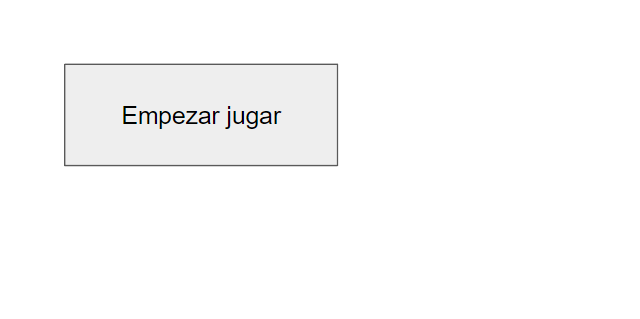
\includegraphics[width=\linewidth]{Imagenes/Eva/C.png}
		\caption{Ejemplo de imagen positivo en solapamiento.}
		\label{fig:C}
	\end{minipage}
	\hfill
	\begin{minipage}{0.45\textwidth}
		\centering
		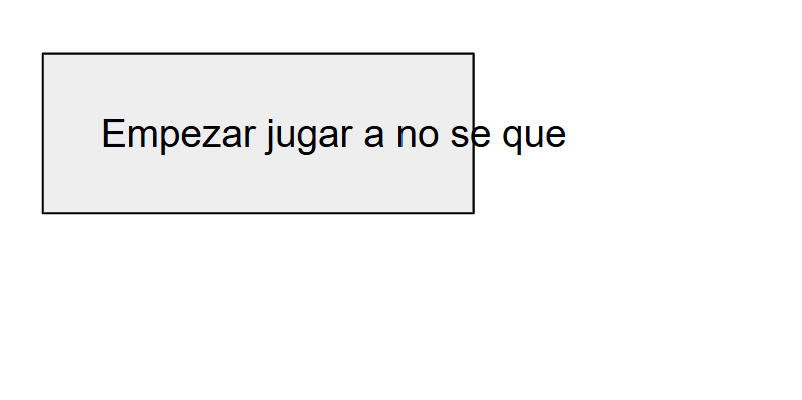
\includegraphics[width=\linewidth]{Imagenes/Eva/F.png}
		\caption{Ejemplo de imagen negativo en solapamiento.}
		\label{fig:F}
	\end{minipage}
\end{figure}
\subsection{Test de truncamiento}
En este test, para el suite de test positivos, se define la cadena del texto esperado y el texto reconocido de forma simétrica comprobando que pasa el test de truncamiento. En el suite de negativos, se define la cadena del texto esperado, y las cadenas del texto reconocido son subcadenas del texto esperado.P.ej :
\begin{itemize}
	\item Texto esperado: Empezar jugar
	\item Texto reconocido: Empezar jug
\end{itemize}
\subsection{Resultado del test de unidad}
Se ejecutan:
\begin{itemize}
	\item Placeholder: 8 casos positivos y 5 casos negativos.
	\item Solapamiento: 2 casos positivos y 2 casos negativos.
	\item Truncamiento: 2 casos positivos y 3 casos negativos.
\end{itemize}
Ejecutando el test de unidad obtenemos que se ha pasado todos los tests, tanto positivos como negativos por lo que podemos llegar a la conclusión de que la implementación de los tests son correctas.


\section{Evaluación de la herramienta}
\label{sec:Evaluación_herramienta}
En esta sección se hará una evaluación de la herramienta comprobando el funcionamiento completo incluyendo los dos modulos de OCR y tests.
El objetivo de esta evaluación es asegurar de que nuestra herramienta es preciso y exacto como ayuda de la parte de LQA.
La metodología de la evaluación es la siguiente:
\begin{enumerate}
	\item Se ha creado una batería de pruebas con 30 imágenes en total. Entre las 30 imágenes, existen \begin{itemize}
		\item 7 errores de solapamiento
		\item 5 errores de truncamiento
		\item 5 errores de placeholders
	\end{itemize}
	Las imágenes de prueba con errores de localización se ha hecho editando sobre imágenes de los juegos sobrescribiendo sobre el contenido original.
	\item Se ejecutará la herramienta propocionando información de estas imagenes y configuración.
	\item Se obtendrá los resultados de las imágenes.
	\item Se generará una matriz de confusión con los resultados obtenidos y esperados.
	\item Se obtendrá información de la matriz de confusión como precisión, falsos positivos y falsos negativos.
\end{enumerate}
En la matriz de confusión: 
\begin{itemize}
	\item Positivo representa que existe un error de localización.
	\item Negativo representa que no existe error de localización.
	\item El valor esperado es el resultado de la herramienta.
	\item El valor real es el valor que realmente es.
	\item Verdadero positivo(TP) indica que hay error y detecta error.
	\item Falso positivo(FP) indica que no hay error pero detecta error. 
	\item Verdadero negativo(TN) indica que no hay error y no detecta error.
	\item Falso negativo(FN) indica que hay error pero no detecta error. 
	\item Exactitud mide el porcentaje de predicciones correctas sobre el total de predicciones. Indica el porcentaje de acierto sobre si existe o no errores de localización en las imágenes.
	
	$Exactitud = \frac{TP + TN}{TP + TN + FP + FN}$
	
	\item Precisión mide el porcentaje de predicciones positivas correctas sobre el total de predicciones positivas. Indica el porcentaje de acierto de detección de errores de localización.
	
	$Precision = \frac{TP}{TP + FP}$
\end{itemize}
el aspecto de la matriz es similar a la tabla \ref{table:mt_ej}

\begin{table}[H]
	\centering
	\begin{tabular}{|c|c|c|c|}
		\hline
		& & Real &   \\
		\hline
		&          & Positivo & Negativo                   \\
		\hline
		Esperado & Positivo & TP& FP \\
		\hline
		& Negativo & 		  FN& TN                \\
		\hline
				&&&\\
		\hline
		&Exactitud&  & \\
		\hline
		&Precisión&  &\\
		\hline
	\end{tabular}
	\caption{Matriz de confusión ejemplo.}
	\label{table:mt_ej}
\end{table}
\begin{table}[H]
	\centering
	\begin{tabular}{|c|c|c|c|}
		\hline
		& & Real &   \\
		\hline
		&          & Positivo & Negativo                   \\
		\hline
		Esperado & Positivo & 14& 2 \\
		\hline
		& Negativo & 		  12& 2                 \\
 		\hline
 						&&&\\
 		\hline
 		&Exactitud& 53.33 & \\
 		\hline
 		&Precisión& 87.5 &\\
 		\hline
	\end{tabular}
	\caption{Matriz de confusión del resultado.}
	\label{table:mt_ori}
\end{table}

Como podemos observar en la tabla \ref{table:mt_ori} se producen 12 falsos negativos(se espera que detecte errores de localización pero la herramienta no lo detecta) y 2 falsos positivos(se esperaba que no exista ningún error de localización pero la herramienta los detecta como error). La cantidad de falsos positivos indica que la herramienta está detectando errores en imágenes donde no debería aparecer errores, esto es un problema para nuestra herramienta ya que nuestro fin es minimizar trabajo de un ser humano y este tipo de error aumenta el trabajo teniendo que evaluar las imágenes cuando en realidad no tiene ningún error. Y los falsos negativos indica que la herramienta no detecta ningún error en la imagen cuando en realidad existen errores lo que también es un problema porque la herramienta trata de reconocer errores para ser corregidos antes de la publicación del juego. Podemos observar que la precisión de la herramienta es alta(87.5\%) pero la exactitud es mediana(53.33\%) por lo cual la herramienta puede estar detectando errores de localización pero mucha de las veces falla en clasificar si una imagen tiene o no error de localización.

Para obtener más detalle de la evaluación, generaremos una matriz de confusión para cada tipo de test.

\begin{table}[H]
	\centering
	\begin{tabular}{|c|c|c|c|}
		\hline
		& & Real &   \\
		\hline
		&          & Positivo & Negativo                   \\
		\hline
		Esperado & Positivo & 3& 4 \\
		\hline
		& Negativo & 		  7& 16                 \\
		\hline
 						&&&\\
		\hline
		&Exactitud& 63.33 & \\
		\hline
		&Precisión& 42.86 &\\
		\hline
	\end{tabular}
	\caption{Matriz de confusión del resultado de solapamiento.}
	\label{table:mt_ori_sol}
\end{table}

\begin{table}[H]
	\centering
	\begin{tabular}{|c|c|c|c|}
		\hline
		& & Real &   \\
		\hline
		&          & Positivo & Negativo                   \\
		\hline
		Esperado & Positivo & 5& 0 \\
		\hline
		& Negativo & 		  20& 5                 \\
		\hline
		 						&&&\\
		\hline
		&Exactitud& 33.33 & \\
		\hline
		&Precisión& 100 &\\
		\hline
	\end{tabular}
	\caption{Matriz de confusión del resultado de truncamiento.}
\label{table:mt_ori_trun}
\end{table}
\begin{table}[H]
	\centering
	\begin{tabular}{|c|c|c|c|}
		\hline
		& & Real &   \\
		\hline
		&          & Positivo & Negativo                   \\
		\hline
		Esperado & Positivo & 0& 5 \\
		\hline
		& Negativo & 		  0& 25                \\
		\hline
		 						&&&\\
		\hline
		&Exactitud& 83.33 & \\
		\hline
		&Precisión& 0 &\\
		\hline
	\end{tabular}
	\caption{Matriz de confusión del resultado de placeholders.}
\label{table:mt_ori_place}
\end{table}
Mirando los resultados de cada test, podemos observar en la tabla \ref{table:mt_ori_sol}, se producen 11 errores(falso positivo + falso negativo) al detectar solapamiento lo cual ha conseguido acertar en 19 imágenes(63.33\% de exactitud) y que de los 7 errores que había, ha conseguido detectar 3(42.86\% de precisión). Sin embargo en las otras dos existen errores graves. En la tabla \ref{table:mt_ori_trun} podemos observar que se detectan 20 casos de falsos negativos que es un valor bastante alto lo que baja la exactitud a un 33.33\%. En la tabla \ref{table:mt_ori_place} observamos que se produce 25 casos de verdaderos negativos y 5 casos de falsos positivos, aunque parezca que tiene buenos resultados, recordamos que existe 5 errores de placeholders solamente, lo cual significa que no ha conseguido detectar ninguno de ellos(0\% de precisión). 
Lo que tienen en común estos últimos dos test es que usan el texto reconocido en la salida del OCR lo cual el problema puede encontrarse allí.

Observando el informe los resultados de salida, de las 30 imágenes de prueba, el porcentaje de similitud de 17 imágenes son menores del 50\% y entre ellas, 14 son 0\%, esto significa que no se esta reconociendo de forma correcta el texto de las imágenes produciendo todo ese error en los tests. Por tanto, aunque en la tabla \ref{table:mt_ori_trun} obtenga una precisión de 100\%, esto puede ser debido al mal reconocimiento de texto produciendo un error de truncamiento y que ``justamente'' en esas imágenes existen error de truncamiento.

Haciendo una investigación del problema, se detecta que el problema puede ser producido en el proceso de preprocesamiento, por lo cual mostramos por salida el resultado de la imagen después del preprocesamiento de la figura \ref{fig:Eva_2} (imagen original) obteniendo el resultado como se muestra en la figura \ref{fig:Eva_2P}.
\begin{figure}[H]
	\centering
	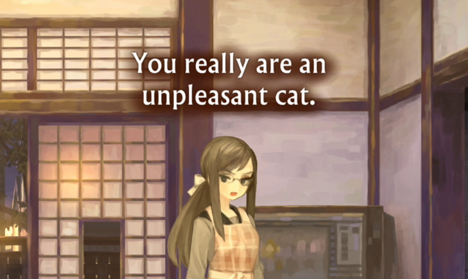
\includegraphics[width = 0.6\textwidth]{Imagenes/Evaluacion_OCR/2.png}
	\caption{Imagen ejemplo de prueba.}
	\label{fig:Eva_2}
\end{figure}
\begin{figure}[H]
	\centering
	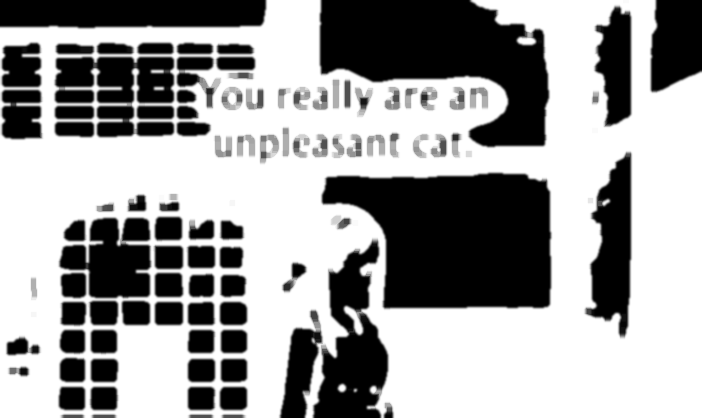
\includegraphics[width = 0.6\textwidth]{Imagenes/Evaluacion_OCR/2_prepro.png}
	\caption{Resultado de la imagen de prueba después de preprocesamiento.}
	\label{fig:Eva_2P}
\end{figure}

Podemos ver que la imagen preprocesada se ve borroso en la parte del texto incluso a ojo humano, por tanto es de lo esperado que el OCR no consiga reconocer el texto de la imagen.
Este problema es debido a que en la sección \ref{sec:Mejoras en el reconocimiento}, la evaluación del CER de los preprocesamientos se ha hecho sin tener en cuenta la distancia levenshtein que fue implementado y evaluado posteriormente del preprocesamiento. El bajo CER que se obtuvo es debido a que el OCR reconocía menos caracteres basura pero sin reconocer el texto. Puede darse el caso de que el OCR reconozca el texto pero con mucha basura, lo que  aumenta el CER, algo que se soluciona aplicando la distancia levenshtein.

Para intentar resolver este problema, evaluaremos la herramienta quitando los preprocesamientos que hagan que la imagen se vea más borroso que son:
\begin{itemize}
	\item Denoising
	\item Blurring
	\item Dilatar y erosionar.
\end{itemize}
\begin{figure}[H]
	\centering
	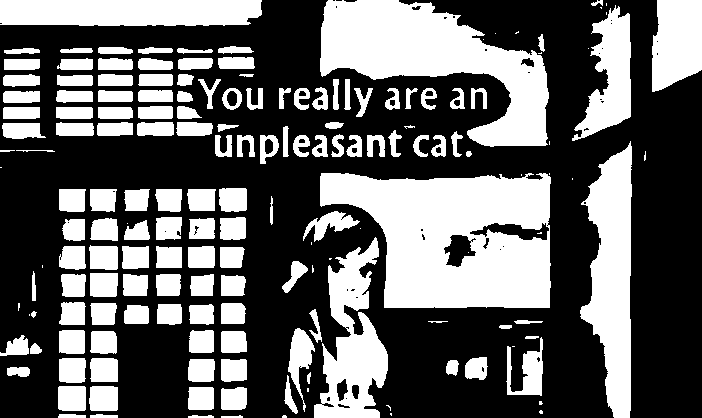
\includegraphics[width = 0.6\textwidth]{Imagenes/Evaluacion_OCR/2_p.png}
	\caption{Resultado de la imagen de prueba después del nuevo preprocesamiento.}
	\label{fig:Eva_2PP}
\end{figure}
Se obtiene la imagen que se muestra en la figura \ref{fig:Eva_2PP} y los siguientes nuevos resultados.
\begin{table}[H]
	\centering
	\begin{tabular}{|c|c|c|c|}
		\hline
		& & Real &   \\
		\hline
		&          & Positivo & Negativo                   \\
		\hline
		Esperado & Positivo & 15& 1 \\
		\hline
		& Negativo & 		  12& 2                \\
		\hline
		 						&&&\\
		\hline
		&Exactitud& 56.67 & \\
		\hline
		&Precisión& 93.75 &\\
		\hline
	\end{tabular}
	\caption{Matriz de confusión del resultado.}
\label{table:mt_pos}
\end{table}
\begin{table}[H]
	\centering
	\begin{tabular}{|c|c|c|c|}
		\hline
		& & Real &   \\
		\hline
		&          & Positivo & Negativo                   \\
		\hline
		Esperado & Positivo & 3& 4 \\
		\hline
		& Negativo & 		  7& 16                \\
		\hline
		 						&&&\\
		\hline
		&Exactitud& 63.33 & \\
		\hline
		&Precisión& 42.86 &\\
		\hline
	\end{tabular}
	\caption{Matriz de confusión del resultado de solapamiento.}
\label{table:mt_pos_sol}
\end{table}

\begin{table}[H]
	\centering
	\begin{tabular}{|c|c|c|c|}
		\hline
		& & Real &   \\
		\hline
		&          & Positivo & Negativo                   \\
		\hline
		Esperado & Positivo & 5& 0 \\
		\hline
		& Negativo & 		  20& 5                \\
		\hline
		 						&&&\\
		\hline
		&Exactitud& 33.33 & \\
		\hline
		&Precisión& 100 &\\
		\hline
	\end{tabular}
	\caption{Matriz de confusión del resultado de truncamiento.}
\label{table:mt_pos_trun}
\end{table}
\begin{table}[H]
	\centering
	\begin{tabular}{|c|c|c|c|}
		\hline
		& & Real &   \\
		\hline
		&          & Positivo & Negativo                   \\
		\hline
		Esperado & Positivo & 1& 4 \\
		\hline
		& Negativo & 		  0& 25                \\
		\hline
		 						&&&\\
		\hline
		&Exactitud& 86.67 & \\
		\hline
		&Precisión& 20 &\\
		\hline
	\end{tabular}
	\caption{Matriz de confusión del resultado de placeholders.}
\label{table:mt_pos_place}
\end{table}
Vemos que no ha mejorado mucho en la matriz de confusión, sin embargo si tenemos en cuenta el porcentaje de similitud como se observa en la tabla \ref{table:simi}, sí que se ha mejorado de forma genérica teniendo 15 imágenes por debajo del 50\% y entre ellas 9 imágenes de 0\%.

También observamos que en algunos casos ha empeorado, como puede ser la imagen 1 que tenía un 85\% y que ahora está a 0\%. 
\begin{table}[H]
	\centering
	\begin{tabular}{lll} 
		Imagen & Antes  & Después \\
		1  & 85.71 & 0      \\     
		2  & 0     & 0      \\  
		3  & 0     & 0      \\  
		4  & 0     & 100    \\  
		5  & 0     & 70.32  \\  
		6  & 0     & 70  \\ 
		7  & 0     & 81.63  \\  
		8  & 91    & 60.60  \\  
		9  & 86.66 & 86.66  \\  
		10 & 53.84 & 57.69  \\  
		11 & 75.67 & 59.35  \\  
		12 & 10.09 & 35.77  \\  
		13 & 54.92 & 54.92  \\  
		14 & 0     & 0      \\  
		15 & 0     & 0      \\  
		16 & 0     & 0      \\  
		17 & 0     & 0      \\  
		18 & 100   & 100    \\    
		19 & 0     & 0      \\     
		20 & 76.92 & 76.92  \\  
		21 & 54.05 & 51.35  \\  
		22 & 0     & 26.60  \\  
		23 & 0     & 35.77  \\  
		24 & 10    & 34.86  \\  
		25 & 69    & 47.88  \\  
		26 & 67    & 54.92  \\  
		27 & 0     & 0      \\  
		28 & 96    & 96     \\  
		29 & 30    & 30.30  \\  
		30 & 96.42 & 94.64  \\  
	\end{tabular}
		\caption{Comparación de porcentaje de similitud entre los dos preprocesamientos.}
	\label{table:simi}
\end{table}
Con esto podemos llegar a la conclusión de que es necesario diferente preprocesamiento dependiendo de las características de las imágenes.
Para ello, se intentará buscar el mejor preprocesamiento para cada imagen. Se ejecutará los siguientes tipos de preprocesamiento:
\begin{itemize}
	\item El preprocesado original de la sección \ref{sec:Mejoras en el reconocimiento}.
	\item El preprocesado mejorado de esta sección.
	\item Escala de grises y ajuste adaptativo de contraste.
	\item Escala de grises y simple thresholding.
	\item Escala de grises solamente.
\end{itemize}
Se aplican distintos métodos de preprocesado teniendo en cuenta que, en algunas imágenes, dicho preprocesado puede empeorar la calidad del reconocimiento, mientras que en otras resulta imprescindible para mejorar los resultados. Por ello, para cada imagen se evaluarán las diferentes opciones de preprocesado y se seleccionará aquella que obtenga el mayor porcentaje de similitud en el reconocimiento del texto.
Se obtiene los siguientes nuevos resultados:
\begin{table}[H]
	\centering
	\begin{tabular}{|c|c|c|c|}
		\hline
		& & Real &   \\
		\hline
		&          & Positivo & Negativo                   \\
		\hline
		Esperado & Positivo & 15& 1 \\
		\hline
		& Negativo & 		  10& 4                \\
		\hline
		&&&\\
		\hline
		&Exactitud& 63.33 & \\
		\hline
		&Precisión& 93.75 &\\
		\hline
	\end{tabular}
	\caption{Matriz de confusión del resultado.}
	\label{table:mt_n}
\end{table}
\begin{table}[H]
	\centering
	\begin{tabular}{|c|c|c|c|}
		\hline
		& & Real &   \\
		\hline
		&          & Positivo & Negativo                   \\
		\hline
		Esperado & Positivo & 4& 3 \\
		\hline
		& Negativo & 		  6& 17                \\
		\hline
		&&&\\
		\hline
		&Exactitud& 70 & \\
		\hline
		&Precisión& 57.14 &\\
		\hline
	\end{tabular}
	\caption{Matriz de confusión del resultado de solapamiento.}
	\label{table:mt_sol_n}
\end{table}

\begin{table}[H]
	\centering
	\begin{tabular}{|c|c|c|c|}
		\hline
		& & Real &   \\
		\hline
		&          & Positivo & Negativo                   \\
		\hline
		Esperado & Positivo & 5& 0 \\
		\hline
		& Negativo & 		  17& 8                \\
		\hline
		&&&\\
		\hline
		&Exactitud& 39.39 & \\
		\hline
		&Precisión& 62.5 &\\
		\hline
	\end{tabular}
	\caption{Matriz de confusión del resultado de truncamiento.}
	\label{table:mt_trun_n}
\end{table}
\begin{table}[H]
	\centering
	\begin{tabular}{|c|c|c|c|}
		\hline
		& & Real &   \\
		\hline
		&          & Positivo & Negativo                   \\
		\hline
		Esperado & Positivo & 1& 4 \\
		\hline
		& Negativo & 		  0& 25                \\
		\hline
		&&&\\
		\hline
		&Exactitud& 86.67 & \\
		\hline
		&Precisión& 20 &\\
		\hline
	\end{tabular}
	\caption{Matriz de confusión del resultado de placeholders.}
	\label{table:mt_place_n}
\end{table}
\begin{table}[H]
	\centering
	\begin{tabular}{lll} 
		Imagen & Antes  & Mejor de cada imagen. \\
		1  & 85.71 & 86      \\     
		2  & 0     & 70      \\  
		3  & 0     & 67      \\  
		4  & 0     & 100    \\  
		5  & 0     & 91  \\  
		6  & 0     & 70  \\ 
		7  & 0     & 89  \\  
		8  & 91    & 91  \\  
		9  & 86.66 & 86.66  \\  
		10 & 53.84 & 65  \\  
		11 & 75.67 & 75.67 \\  
		12 & 10.09 & 38  \\  
		13 & 54.92 & 83  \\  
		14 & 0     & 8      \\  
		15 & 0     & 73      \\  
		16 & 0     & 88      \\  
		17 & 0     & 76      \\  
		18 & 100   & 100    \\    
		19 & 0     & 65     \\     
		20 & 76.92 & 76.92  \\  
		21 & 54.05 & 70  \\  
		22 & 0     & 29  \\  
		23 & 0     & 38  \\  
		24 & 10    & 34.86  \\  
		25 & 69    & 76  \\  
		26 & 67    & 63  \\  
		27 & 0     & 45      \\  
		28 & 96    & 96     \\  
		29 & 30    & 79  \\  
		30 & 96.42 & 96.42  \\  
	\end{tabular}
	\caption{Comparación de porcentaje de similitud entre el preprocesado original y los mejores de cada imagen.}
	\label{table:simi_n}
\end{table}
Como podemos observar en las tablas \ref{table:mt_n}, \ref{table:mt_sol_n} y \ref{table:mt_trun_n}, se vuelve a mejorar un poco los resultados en cuanto la exactitud. El porcentaje de similitud en este caso ya no hay ningún valor a 0\% y solamente hay 6 imágenes con valores inferiores al 50\% como podemos ver en la tabla \ref{table:simi_n}. Este proceso de preprocesamiento específico para cada imagen no es trivial por lo que es necesario en un futuro obtener características de la imágenes y aplicar determinadas técnicas de preprocesamiento según las características.

Como se puede observar en las Tablas \ref{table:mt_n}, \ref{table:mt_sol_n} y \ref{table:mt_trun_n}, se aprecia una ligera mejora en los resultados de exactitud. En cuanto al porcentaje de similitud, ya no se presentan valores del 0\%, y únicamente seis imágenes registran valores inferiores al 50\%, como se detalla en la Tabla \ref{table:simi_n}. Este resultado indica que el uso de un preprocesamiento específico por imagen contribuye a mejorar el rendimiento del sistema. Sin embargo, este proceso no es trivial, por lo que en trabajos futuros sería recomendable extraer características relevantes de cada imagen y aplicar técnicas de preprocesamiento adaptadas a dichas características.

En conclusión, la precisión y exactitud de la herramienta se sitúan en un nivel intermedio y son claramente mejorables. Una de las principales limitaciones es que el OCR no logra reconocer el texto de forma completamente precisa, lo que sugiere que es necesario optimizar el preprocesamiento para mejorar el rendimiento del reconocimiento. Una posible línea de mejora sería el entrenamiento del modelo OCR con fuentes específicas del videojuego, ya que hasta ahora se ha utilizado únicamente el modelo por defecto de Tesseract.

\section{Conclusión}
En este capítulo se ha llevado a cabo la evaluación del módulo de OCR, del módulo de tests y, finalmente, de la herramienta en su conjunto. En la evaluación del módulo de OCR, Tesseract ha demostrado ser la opción más adecuada para el caso de uso planteado. Con el fin de mejorar el reconocimiento de texto, se han aplicado técnicas como el preprocesamiento de imágenes, que facilita la detección de texto, y el uso de la distancia de Levenshtein para medir la similitud entre cadenas, lo cual permite filtrar caracteres irrelevantes o erróneos.

Para evaluar el módulo de tests se ha desarrollado una prueba unitaria específica, cuyos resultados han sido satisfactorios, demostrando el correcto funcionamiento del sistema de validación.

En cuanto a la evaluación global de la herramienta, los resultados obtenidos reflejan un rendimiento aceptable pero claramente mejorable. La principal limitación detectada radica en el reconocimiento textual por parte del OCR. Para mitigar este problema, se propone como línea de mejora futura la adaptación del preprocesamiento en función de las características de cada imagen, así como el entrenamiento de un modelo OCR específico para la fuente utilizada en el videojuego, en lugar de depender exclusivamente del modelo por defecto.